\documentclass[11pt]{article}

\usepackage[utf8]{inputenc}
\usepackage{amsmath, amssymb}
\usepackage{graphicx}
\usepackage{booktabs}
\usepackage{geometry}
\usepackage{hyperref}
\usepackage{natbib}
\geometry{letterpaper, margin=1in}
\bibliographystyle{apalike}

\title{Informational Order Flow and the Term Structure of Price Impact:\\ The Permanent Footprint of Concealed Execution\\ and Overnight Efficiency}
\author{Nicholas Jiang}
\date{July 2026}

\begin{document}

\maketitle

\begin{abstract}
Distinguishing temporary mechanical price impact from permanent informational price discovery is a central challenge in market microstructure. This paper investigates the \emph{lifecycle of information} in aggressive order flow: how the directional content of intraday order-submission bursts---temporally clustered, same-side executions---is reflected in prices, and how quickly an efficient market absorbs it. A caution on attribution belongs at the outset. We observe anonymous message-level executions, not trader identities: we have no parent-order data, no broker records, and no linkage to institutional holdings. The median burst is roughly $320$ shares completing in seconds, which is consistent with a fragment of an institutional execution schedule but equally consistent with retail smart-order-router fragments, market-maker hedging, or high-frequency liquidity provision. We therefore describe bursts as \emph{clustered aggressive executions} and make no claim about who submits them; where the metaorder literature is invoked, it is as a point of comparison for magnitudes, not as an identification of our objects with parent orders. Using event-by-event LOBSTER limit-order-book data for a 482-name NASDAQ universe over 2022--2026, reconstructed directly from the raw ITCH message stream, we trace the burst footprint across horizons spanning seconds to the overnight close, under look-ahead controls enforced architecturally throughout the pipeline.

The central finding is that this impact is \emph{permanent, not transient}, and that it is carried specifically by \emph{aggressive} concealment. Hidden-execution bursts with an identifiable aggressor---those executing away from the midpoint---move price by a mean $+2.1$ bps over three minutes across the full 474-name cross-section, and the markout is then flat ($+2.2$ at fifteen and thirty minutes, and a placebo-netted $+2.1$ bps to the close). Price does not return toward the pre-burst mid at any horizon we measure. The roughly half of hidden volume that executes \emph{at} the midpoint, by contrast, carries no such footprint---a small negative markout consistent with uninformed liquidity provision---so the permanent footprint is a property of aggressive hidden execution, not of hidden execution indiscriminately (Appendix~\ref{sec:bifurcation}). This informed footprint is the adverse-selection component of the spread measured directly. On the \citet{huangstoll1997} accounting it is $51\%$ of the effective half-spread a taker pays and $32\%$ of the quoted half-spread---a substantial share of trading costs, not a small one. It remains, however, strictly \emph{inside} the spread, which is what the Glosten--Milgrom mechanism predicts and what makes the footprint uncrossable rather than tradeable; the barrier to monetizing it is the cost of crossing, not the size of the signal. Consistent with permanence rather than decay, the relation \emph{does not extend past the trading day}: the close-to-open information coefficient is $-0.001$ ($t=-0.4$), an economic and statistical zero, meaning no further predictability---not that the earlier move reverts. Decomposing the daily return into its overnight and intraday sessions does not change this: on the primary panel no session-level leg is distinguishable from zero.

The measurement rests on two now-standard safeguards rather than novel methods: the forward-looking decay filter $D_b$ (definitionally the 1--10 minute forward markout) is excluded from the predictive feature set and from any intraday evaluation inside its own window; and inference is conducted at the day level with date-clustered errors. The paper's contribution is therefore empirical rather than methodological: a precise, cross-sectional characterization of informational order flow as a real, intraday-persistent but sub-spread phenomenon that the overnight market prices out with efficiency, together with the identification of hidden-execution clustering as the one burst reconstruction---among Hawkes, order-flow-imbalance, and book-resilience alternatives---carrying a robust informed footprint. A conditional cross-sectional asymmetry is also documented---reversal concentrated in tick-constrained names and undetectable in large-tick ones---and its mechanism is set out, but establishing whether it is deployable requires a calibration period disjoint from the evaluation period and a point-in-time universe, and we defer that measurement to such a design.
\end{abstract}

\section{Introduction}
Financial markets are driven by heterogeneous trading activity. While some orders primarily provide or consume liquidity and generate only short-lived price effects, others reflect fundamental information that leads to persistent, permanent price changes. The theoretical foundations of informational price discovery have long established that informed traders gradually incorporate private signals into prices to avoid excessive market impact \citep{kyle1985}. Empirical evidence supports this, demonstrating that certain classes of traders systematically trade in the direction of permanent price changes, contributing to price discovery rather than transient mechanical pressure \citep{brogaard2014, hasbrouck1991}.

A key empirical regularity in equity markets is the strong persistence of order flow over extended horizons. This persistence is overwhelmingly driven by order splitting, a process where a single institutional investor gradually executes a large trading intention through a sequence of same-side orders \citep{toth2015}. A large recent literature formalizes the predictive content of this signed order flow through order-flow imbalance and its deep-learning extensions \citep{cont2014,kolm2023,lucchese2024}, through cross-asset propagation \citep{cont2023crossimpact}, and---most directly related to the present work---through a \emph{conditional} decomposition of trade flow into typed order-imbalance predictors of the cross-section of daily returns \citep{cont2023clientflow,lrc2024,sitaru2023}. The burst construction studied here can be read as one such conditioning: an event-time aggregation of same-side aggressive flow into discrete, geometrically filtered clusters. Furthermore, the price impact of trades is well known to be \emph{transient}---decaying over time as liquidity replenishes, as formalized by propagator and supply/demand-dynamics models of impact \citep{bouchaud2004,obizhaeva2013}---which both necessitates that large meta-orders be executed through hidden or fragmented bursts to minimize execution costs \citep{moro2009, bucci2019} and frames the central question of this paper: how much of a burst's impact is transient versus permanent, and over what horizon. The overnight component of returns, in particular, behaves differently from the intraday component \citep{lou2019}, which motivates measuring the burst footprint separately at intraday and overnight horizons. Motivated by these dynamics, this paper studies whether intraday order submission behavior can be used to identify longer-horizon informational order flow. Note that while resting limit order submissions establish the background liquidity structure, the empirical scope of this paper focuses on aggressive order executions (marketable trades) that actively consume this liquidity; a first pass at clustering \emph{passive} limit-order submissions is reported as a negative control in Appendix~\ref{sec:appendix_passive}, with a fuller treatment left to future work.

This paper approaches that question as a first-principles investigation into how information in order flow is \emph{impounded and then priced}, and organizes its evidence around a single scientific thesis: bursts that conceal \emph{aggressive} execution carry genuine informed directional pressure into prices; that pressure is impounded \emph{permanently} within minutes and thereafter neither grows nor reverts; and by the overnight horizon it generates no further predictability, the market having priced it efficiently. The empirical object is therefore not a trading strategy but the \emph{term structure of a burst's price impact}---how a measurable footprint appears within minutes, persists without reverting through the trading day, and leaves no predictability across the overnight clearing return.

To answer it without the confounds that plague high-frequency backtests, the primary subject of study is the full cross-section from the outset: a fixed, start-of-sample list of 482 high-liquidity NASDAQ-traded names spanning 2022--2026, of which 438 are strictly out-of-sample relative to a small parameter-tuning set. Cross-sectional breadth---rather than a hand-picked showcase of high-volatility single names---is what lets us separate a real informed footprint from selection and pseudo-replication artifacts, and it is where every quantitative claim in the paper is made. Throughout, we define informational order flow as trading activity whose directional price impact persists beyond the immediate mechanical bounce, and we measure that persistence directly via a multi-horizon markout panel rather than inferring it from realized backtest P\&L. Two design commitments make the measurement credible and are stated here because they shape everything that follows: any quantity defined on \emph{forward} prices (notably the decay filter $D_b$ below) is quarantined to ex-post impact measurement and never enters a predictive feature set, and the day, not the individual burst, is treated as the unit of statistical inference.

\section{Data and Limit Order Book Reconstruction}
\label{sec:data}
Our empirical analysis relies on ultra-high-frequency, event-by-event limit order book (LOB) data provided by LOBSTER (Limit Order Book System, the Efficient Reconstructor), reconstructed directly from the NASDAQ (ITCH) message stream. The primary and near-exclusive subject of study is the \emph{full cross-section}: a \emph{fixed list} of 482 high-liquidity names traded on NASDAQ (a mix of NASDAQ- and NYSE-listed common stocks and ETFs, reconstructed from the NASDAQ book), of which 438 are strictly out-of-sample relative to the parameter-tuning set. A small \emph{tuning set} of four high-volatility single names---NVIDIA (NVDA), Tesla (TSLA), JPMorgan Chase (JPM), and Morgan Stanley (MS)---serves a strictly circumscribed role: it is the set on which the physical burst-detection parameters are calibrated (Section~\ref{sec:optuna}) and, later, a source of illustrative microstructure detail. Because these four names define the tuning set, they are in-sample by construction and carry no evaluative inference; all quantitative results are reported on the out-of-sample cross-section. The intraday markout measurements involve no tuned strategy parameters and no forward evaluation window. The membership rule and its survivorship limitation must be stated carefully. The list is fixed by a liquidity screen among the names that the LOBSTER archive stages, and---as we document in Section~\ref{sec:integrity}---the ticker set that archive stages is itself survivor-conditioned: names that later delisted are silently absent from the files we can reach rather than present as truncated series. The universe is therefore not point-in-time, and the affirmative reversal is exposed to a delisting bias that we quantify and bound in Section~\ref{sec:integrity}---but cannot remove within our data access, since the delisted names' order flow is not retrievable from the staged archive (whether it is retrievable from the vendor at all is a question we have not settled; see Section~\ref{sec:integrity}). Daily open and close prices used for overnight and close-to-close returns are sourced from the Polygon/Massive consolidated daily feed; corporate-action (split/dividend) adjustment of these prices, which is first-order in the low-priced names that carry the affirmative result, is treated explicitly as a data-integrity check rather than assumed. Because LOBSTER reconstructs the NASDAQ book only, the fraction of consolidated volume captured varies by name (notably for the NYSE-listed financials JPM and MS); this venue-coverage caveat is stated in the cross-sectional analysis (Section~\ref{sec:venue}).

Standard vendor-aggregated data often introduces temporal blurring that obscures high-frequency signal integrity. To prevent this, we process the raw Level 3 LOBSTER message stream directly using a bespoke C++ data processor. By tracking the exact bid and ask price levels, resting depth, and microsecond timestamps, this procedure allows us to observe the precise liquidity conditions facing an order at the exact moment of submission.

\subsection{Data Summary Statistics}
Table \ref{tab:data_summary} presents summary statistics for the four tuning names, which span the microstructural range that governs the paper's central tick-regime result. A critical distinction emerges from the average spread column. NVDA's average quoted spread of \$0.104 spans approximately 10 minimum price increments (ticks), meaning that a moderately aggressive institutional order can sweep through multiple resting price levels before being fully absorbed. This multi-level sweep generates the sharp, identifiable burst signatures that the detection algorithm relies on. By contrast, a tick-constrained name such as AAPL---whose spread is typically locked at the \$0.01 minimum tick, with massive queued depth at the best bid and ask---absorbs even large institutional orders passively at a single price level, producing no detectable multi-level sweep. This large-tick-versus-tick-constrained axis, established here on familiar names, becomes the organizing variable of the cross-sectional analysis (Section~\ref{sec:reversion}).

\begin{table}[htbp]
\centering
\resizebox{\textwidth}{!}{
\begin{tabular}{llrrrrr}
\toprule
\textbf{Ticker} & \textbf{Period} & \textbf{Trading Days} & \textbf{Total Raw Bursts} & \textbf{Bursts/Day} & \textbf{Avg Daily Burst Vol (sh.)} & \textbf{Avg Spread (\$)} \\
\midrule
NVDA & 2023--2024 & 499 & 894,343 & 1,792 & 12,083,125 & 0.1039 \\
TSLA & 2023--2024 & 499 & 757,120 & 1,517 & 11,702,121 & 0.0346 \\
JPM  & 2023--2024 & 499 & 1,251,679 & 2,508 & 993,261 & 0.0298 \\
MS   & 2023--2024 & 499 & 1,108,679 & 2,222 & 850,519 & 0.0211 \\
\bottomrule
\end{tabular}
}
\caption{Data summary statistics for the four parameter-tuning names, chosen to span the tick-structure range (wide-tick NVDA to tick-constrained MS). \emph{Avg Daily Burst Vol} is the average daily aggregate \emph{burst} volume (shares)---the volume captured by the detector, not consolidated ADV, which for the NYSE-listed names (JPM) is roughly an order of magnitude larger. Avg Spread is the mean time-weighted quoted spread at burst initiation. These four names define the Optuna tuning set and are in-sample by construction; they carry no evaluative inference, and all reported results are on the 438-name out-of-sample cross-section.}
\label{tab:data_summary}
\end{table}

\section{Burst Formulation and Parameterization}
\label{sec:burstdef}
Because single, isolated order submissions are highly noisy and rarely informative at horizons beyond a few seconds, we aggregate temporally clustered orders into discrete ``bursts.'' For each burst $b$, we define its start time $t_{b}$, reference mid-price $m_{t_{b}}$, and its signed aggregate volume:
\begin{equation}
Q_{b} = \sum_{j \in b} side_{j} q_{j}
\end{equation}
where $side \in \{+1, -1\}$ denotes a buy or sell order. These reconstructed bursts constitute the fundamental unit of analysis. That they are genuine structures rather than artifacts of arrival-rate clustering is verified directly (Appendix~\ref{sec:audit}): the observed count of same-side clustered bursts exceeds an \emph{inhomogeneous}-Poisson null matched to each name's empirical intraday intensity profile by a median $z$ of $47$ (and a homogeneous null by $z$ of $87$), rejecting the Poisson null on $100\%$ of name-days.

To construct our dataset from the reconstructed limit order book, we evaluate two distinct clustering methodologies governed by physical control parameters to isolate algorithmic intent from retail noise:

\begin{itemize}
    \item \textbf{Strict Silence Threshold ($\Delta t_{silence}$)}: Our baseline approach where a burst rigidly terminates if the limit order book experiences inactivity exceeding a specific temporal limit (e.g., 0.5s, 1.0s, or 2.0s). 
    \item \textbf{Hawkes Process Intensity ($\lambda(t)$)}: A dynamic behavioral model where burst survival is dictated by a self-exciting point process. The conditional intensity function evolves as:
    \begin{equation}
    \lambda(t) = \mu + \sum_{t_k < t} \alpha \, e^{-\beta(t - t_k)}
    \end{equation}
    where $\mu$ is the background intensity, $\alpha$ controls the magnitude of the excitation from each prior event at time $t_k$, and $\beta$ governs the exponential decay rate. In our implementation, we fix $\beta=1.0$ and $\alpha=0.5$, so each incoming trade spikes the intensity by 0.5, which then decays exponentially with a half-life of $\ln 2 / \beta \approx 0.69$s. A burst remains active as long as $\lambda(t)$ exceeds a background intensity threshold $\lambda_{\min}$. We denote each configuration as $\beta$\textsubscript{$\beta$}$\lambda$\textsubscript{$\lambda_{\min}$}; for example, $\beta_{1.0}\lambda_{0.3}$ indicates $\beta=1.0$ with a minimum intensity threshold of 0.3. This replaces rigid silence cutoffs with a fluid structural definition that naturally bridges microscopic liquidity gaps.
    \item \textbf{Fractional Sweep Volume ($vol\_frac$)}: Dynamically establishes the baseline size for a candidate burst, requiring the aggregate burst volume to exceed a specific fraction of the asset's 14-day trailing Average Daily Traded Volume (ADV). Crucially, this ADV is computed strictly using executed trades (LOBSTER Types 4 and 5), insulating the fractional threshold from the artificial inflation of high-frequency quote-stuffing and rapid cancellations.
    \item \textbf{Directional Consistency Ratio ($dir\_thresh$)}: Enforces that a minimum proportion of the events within the cluster must be on the same side of the book (e.g., $> 70\%$).
    \item \textbf{Volume Ratio ($vol\_ratio$)}: Limits the allowable opposing volume to a fraction of the dominant side's volume.
    \item \textbf{Short-Horizon Decay Filter ($\kappa$)}: Retains bursts where the structural decay measure exceeds a threshold, $D_b \geq \kappa$. The \textbf{peak impact} of a burst is defined as the maximum absolute mid-price displacement achieved during the burst lifetime:
    \begin{equation}
    \text{PeakImpact}(b) = \max_{t \in [t_b, t_b^{\text{end}}]} |m_t - m_{t_b}|
    \end{equation}
    The \textbf{decay metric} $D_b$ then measures how much of this displacement persists over the 1--10 minute forward window. The canonical definition used throughout the pipeline is the average directional markout from the burst-termination mid $M_{\text{end}}$,
    \begin{equation}
    D_b = \frac{1}{3}\sum_{\tau\in\{1,5,10\}\text{m}} \text{side}_b \times (M_{\tau} - M_{\text{end}}),
    \label{eq:db}
    \end{equation}
    normalized by $\text{PeakImpact}(b)$ where a scale-free ratio is required. A large positive $D_b$ indicates that the mid-price has held or extended the burst's displacement; a value near 0 indicates full mean-reversion. The $\kappa$ filter retains only bursts with $D_b\ge\kappa$.

    \textbf{$D_b$ is an ex-post impact metric, firewalled from prediction by construction.} $D_b$ is, definitionally, the 1--10 minute forward markout of a burst; it is realized only \emph{after} the burst terminates and cannot exist at the prediction instant. We therefore treat it strictly as an instrument for \emph{measuring} realized price impact after the fact, and we impose an architectural firewall that excludes $D_b$ and every quantity derived from it from the predictive online-SGD feature set (Section~\ref{sec:features}). The exclusion is enforced architecturally in the pipeline, and we verify that it is immaterial to the conclusion: re-estimating the overnight strategy with every $D_b$-derived feature removed leaves its (null) result essentially unchanged (mean per-name Sharpe $-0.28$ versus $-0.20$; Appendix~\ref{sec:audit}). Its only two admissible uses are (i) as the ex-post decay measurement in the markout analysis and (ii) as a filter applied \emph{strictly to the trailing training window}, never to a same-day prediction candidate. Because $D_b$ is itself the forward markout, any intraday horizon lying inside its own window must be evaluated ungated ($\kappa=0$; Section~\ref{sec:markout}). A live burst ending near the close, moreover, realizes $D_b$ up to ten minutes later---after the 3:50/3:55~PM market-on-close cutoff---so $D_b$ could not be acted upon even if one wished to. Enforcing this separation in the deployed pipeline is what keeps the intraday markout measurements free of forward information.
\end{itemize}

Crucially, when predicting short-horizon permanence (e.g., 1-minute or 3-minute targets), $\kappa$ is strictly set to 0. The decay filter $D_b$ inherently relies on observing the price trajectory at $t+10$ minutes. Applying a $\kappa > 0$ threshold to short-horizon targets would introduce a severe look-ahead bias, as the filter's observation window would extend beyond the prediction horizon itself. Consequently, short-horizon bursts must be evaluated solely on their initial physical and behavioral footprints without relying on post-burst decay gating.

\textbf{Why Short-Horizon Targets Are Excluded from Phase III.} While the initial Optuna sweep evaluated both short-horizon targets (e.g., $cls\_1m$, achieving AUC $> 0.64$) and long-horizon targets ($cls\_clop$), the Phase III execution pipeline exclusively targets the overnight horizon for two reasons. First, short-horizon predictions require immediate intraday execution: to capture a predicted 1-minute or burst-to-close movement, the strategy would need to enter a position within seconds of burst detection and exit minutes later, requiring a fundamentally different execution architecture supporting multiple simultaneous intraday positions with per-burst sizing. This stands in contrast to the MOC/MOO framework, which aggregates all signals into a single daily trade. Second, the short-horizon AUC advantage is mechanically inflated by the $D_b$ look-ahead constraint: because $\kappa=0$ is forced for short targets, the pipeline evaluates a much larger and noisier burst universe, making the high AUC less economically actionable after transaction costs. The overnight target, by contrast, permits rigorous $\kappa$-gating and produces a concentrated, high-conviction signal compatible with large-order execution.

\section{Signal Construction}
\label{sec:signal}
The physical burst-detection parameters are calibrated once on the four-name tuning set, and each classified burst is aggregated into a daily net burst-flow imbalance per name; this daily signal is the input to every empirical result below. The full construction---the Optuna calibration of the detection parameters (Appendix~\ref{sec:mlpipeline}), the execution-fingerprint features (Section~\ref{sec:features}), and the online linear (SGD) model used to gate and score bursts---is deferred to Appendix~\ref{sec:mlpipeline}, because the paper's own baselines (Section~\ref{sec:baselines}) show that the linear model adds nothing over the raw net flow: the deployable content is the \emph{sign of daily net burst order flow}, not the model. We therefore keep the body focused on the empirical measurements and treat the pipeline as signal-construction detail.

\section{Feature Engineering and Impact Measurement}
\label{sec:features}
Upon the termination of a classified burst, we extract a rich, high-dimensional execution fingerprint. Beyond standard Limit Order Book State metrics (Spread, Imbalance, Depth Ratio) and Temporal Dynamics, we incorporate specific algorithmic footprints such as Trade-Size Variance, Round Lot Percentages, and Pre-burst Quote Depletion.

To quantify the true economic footprint of a burst and how much of its initial price displacement persists at longer horizons $\tau$, we utilize a Transformed Volume-Scaled Impact (VSI):
\begin{equation}
VSI(b; \tau) = \text{arcsinh} \left( Q_{b} \times \text{side}_{b} \times (P_{\tau} - m_{t_{b}}) \right)
\end{equation}

To prevent denominator instability inherent in ratio-based metrics during superficial algorithmic pinging, we eschew traditional permanence ratios in favor of this Transformed Volume-Scaled Impact. By scaling the raw directional price displacement by the capital deployed ($Q_b$), we control metric explosion, and the $\text{arcsinh}$ transform compresses heavy-tail outliers into a regression-friendly domain.

\textbf{Target base and tradability.} A subtlety that matters for the overnight target: when the reference mid $m_{t_b}$ is the \emph{burst-start} mid, the reg\_clop target $\text{side}_b\times(\text{Open}_{t+1}-m_{t_b})$ folds in the burst's own contemporaneous impact and the burst-to-close drift, both realized before any market-on-close entry and therefore unearnable. Measured instead from the close mid $M_{\text{end}}$---the tradable close-to-open return---the same predictive rank correlation collapses roughly fivefold and, once clustered by date, to a statistical zero (Section~\ref{sec:breadth}). The predictive $\rho$ reported below for the burst-start base should thus be read as an upper bound on the earnable association, not the tradable quantity.

\subsection{Feature Importance and Model Interpretability}
Since the \texttt{SGDRegressor} is a linear model operating on standardized features, its learned coefficients quantify each feature's marginal contribution to predicted permanence. Across both NVDA and TSLA, one feature dominates: \texttt{Direction} (standardized coefficient $\approx +5.0$ for NVDA, $+4.0$ for TSLA), roughly seventy times the next-largest loading. In other words the fitted model is, to first order, ``follow the burst side''---which raises the question, addressed by the Direction-only ablation in Section~\ref{sec:breadth}, of whether the remaining features earn their place at all. The next-largest loadings are \texttt{PeakImpact} (coef $\approx -0.06$), \texttt{TradeCount}, and \texttt{Duration}, all evaluated at burst termination and admissible as prediction-time features. Consistent with the firewall of Section~\ref{sec:burstdef}, the forward-looking decay measure $D_b$ (Eq.~\ref{eq:db}) is \emph{not} among the predictive features: it is realized only after the burst (and, near the close, after the MOC cutoff), so it is confined to ex-post impact measurement and excluded from the deployed model. Two caveats attach to this ranking. First, a diagnostic fit that \emph{does} admit $D_b$ ranks it second (coef $\approx +0.07$)---an illustration of why the firewall matters, since an unconstrained optimizer would happily lean on the forward markout. Second, these coefficients are estimated on the in-sample tuning names; at cross-sectional scale (Section~\ref{sec:breadth}) the deployed overnight regressor's prediction is in fact \emph{anti}-correlated with the burst side, so the ``follow-the-side'' reading does not survive out of sample.

\section{Parameter Calibration and the Tick-Regime Hypothesis}
\label{sec:empirical}
Before turning to the cross-section, this section documents two things established on the tuning set: the regression-aligned procedure by which the physical burst parameters are calibrated, and the microstructure hypothesis---that tick structure governs the \emph{sign} of a burst's forward return---that organizes the out-of-sample analysis. No single-name trading performance is reported or relied upon; the four tuning names are in-sample by construction and serve only to fix parameters and to motivate the hypothesis that the 438-name out-of-sample cross-section (Sections~\ref{sec:breadth}--\ref{sec:reversion}) then tests.

\subsection{The Necessity of Filtering}
Naive, unconditional burst-following generates negative expected value: executing on every detected burst yields negative per-trade expectancy, driven by immediate bid--ask reversion and the large volume of non-informational algorithmic pinging (the look-ahead-free intraday markout net of the spread is $-3.5$ to $-7.7$ bps per burst; Section~\ref{sec:markout}). The physical filters (Table~\ref{tab:filter_cascade}) compress the raw burst stream by one to two orders of magnitude---for NVDA to roughly a quarter of raw bursts, for TSLA to under one percent. This compression shows that \emph{some} filtering is necessary to avoid the reversion drag; it does \emph{not}, by itself, establish that the surviving signal is informative---a distinction the cross-sectional markout and breadth analyses (Sections~\ref{sec:markout}--\ref{sec:breadth}) make good on.

\subsection{Regression-Aligned Optimization and Empirical Resolution}
To systematically bridge the disconnect between predictive capacity and economic tradability, we implemented a regression-aligned hyperparameter sweep. This framework addresses three critical structural traps that plague standard machine learning backtests in high-frequency regimes:
\begin{itemize}
    \item \textbf{The Sparsity Exploit:} Optimization algorithms tasked with maximizing standard regression correlations quickly exploit dataset sparsity. By shrinking the dataset to an extreme degree, the optimizer can filter out 99.9\% of bursts, leaving a tiny sample where the correlation approaches 1.0. To prevent this, we applied a confidence-scaled scoring metric: $Score = \rho \times \min(1, N_{test}/500)$, alongside a hard minimum floor of 200 total bursts.
    \item \textbf{Fat-Tail Outliers:} Financial return series are characterized by massive fat-tail events. Standard Mean Squared Error (MSE) forces the model to overfit these extreme outliers. We replace MSE with the Spearman rank correlation coefficient ($\rho$), evaluating relative order ranks rather than absolute magnitudes.
    \item \textbf{Model Alignment:} The Optuna sweep evaluates candidate physical parameters using the exact same machine learning pipeline deployed in execution: an \texttt{SGDRegressor} with Huber loss ($\epsilon=1.35$).
\end{itemize}

Table \ref{tab:optuna_regression} outlines the optimal physical parameters discovered by this regression-aligned sweep. The resulting Spearman correlations range from 0.088 to 0.199 with nominally minuscule $p$-values. Two caveats, developed in Sections~\ref{sec:markout}--\ref{sec:breadth}, gut the apparent significance and are stated here so the table is not over-read. First, these $p$-values (e.g.\ JPM's $9.3\times10^{-126}$) treat $\sim$$10^5$ per-burst observations as independent; because all same-day bursts share one overnight label, the effective sample size is the number of \emph{days}, and date-clustering the identical statistic collapses the significance by more than an order of magnitude. Second, the target is measured from the burst-start mid, so $\rho$ overstates association with the tradable close-to-open return by roughly fivefold (Section~\ref{sec:features}); on the tradable, date-clustered target the correlation is statistically zero. The numbers in Table~\ref{tab:optuna_regression} are thus best read as in-sample, pseudo-replicated upper bounds, not evidence of tradable predictability.

\begin{table}[htbp]
\centering
\begin{tabular}{llccccccc}
\toprule
\textbf{Ticker} & \textbf{Target} & \textbf{Best Hawkes} & \textbf{Spearman $\rho$} & \textbf{p-value} & \textbf{$vol\_frac$} & \textbf{$dir\_thresh$} & \textbf{$vol\_ratio$} & \textbf{$\kappa$} \\
\midrule
NVDA & reg\_clop & $\beta_{1.0}\lambda_{0.3}$ & 0.196 & 0.0 & $6.45 \times 10^{-5}$ & 0.509 & 0.583 & 0.824 \\
TSLA & reg\_clop & $\beta_{1.0}\lambda_{0.3}$ & 0.094 & $3.0 \times 10^{-7}$ & $3.30 \times 10^{-3}$ & 0.568 & 0.599 & 1.736 \\
JPM & reg\_clop & $\beta_{1.0}\lambda_{0.3}$ & 0.049 & $9.3 \times 10^{-126}$ & $1.00 \times 10^{-5}$ & 0.561 & 0.570 & 0.200 \\
MS & reg\_clop & $\beta_{1.0}\lambda_{0.3}$ & 0.125 & $1.0 \times 10^{-3}$ & $4.94 \times 10^{-3}$ & 0.902 & 0.018 & 1.399 \\
\bottomrule
\end{tabular}
\caption{Regression-aligned Optuna sweep results (in-sample tuning names). The objective maximizes confidence-scaled Spearman rank correlation evaluated with the backtest \texttt{SGDRegressor}. The reported $p$-values are per-burst and pseudo-replicated (effective $N=$ number of days); the target is measured from the burst-start mid and overstates tradable association---see the text and Sections~\ref{sec:markout}--\ref{sec:breadth}.}
\label{tab:optuna_regression}
\end{table}

\subsection{The Tick-Regime Hypothesis: Tick Structure Governs the Sign of the Signal}
\label{sec:synthesis}
The tuning-set microstructure motivates the hypothesis that the cross-section tests. The relevant axis is not signal-versus-noise but the \emph{sign} of the burst--return relation, and the hypothesis is that this sign is governed by tick structure.

\textbf{Detection vs.\ direction.} The geometric sweep detector fires less cleanly in tick-constrained names: with the spread locked at the \$0.01 tick and heavy queued depth, aggressive meta-orders churn at the inside quote rather than sweeping multiple levels, so raw burst \emph{detection} is noisier there than in large-tick names like NVDA/TSLA. But detection difficulty is not the same as absence of a tradable relation. What we hypothesize changes with tick regime is the sign of the subsequent return: in \emph{large-tick} names a directional burst is more likely to carry and continue, whereas in \emph{tick-constrained} names the inside queue is a binding constraint and aggressive flow tends to overshoot and mean-revert as liquidity replenishes. Trading a tick-constrained name as \emph{momentum} would then be trading the wrong side of a reversal.

This is a hypothesis, not a result: it is stated here because the tuning-set microstructure suggests it, and it is put to a strict out-of-sample test---the cross-sectional sign analysis (Section~\ref{sec:signsign}) and the conditional-reversal strategy (Section~\ref{sec:reversion})---on the 438 names that played no role in forming it. That the sign asymmetry is precisely what the full universe delivers is the paper's one affirmative empirical finding.

\section{The Multi-Horizon Markout Panel}
\label{sec:markout}
The markout decay curve---the directional post-burst return at a panel of forward horizons---is the natural first-class diagnostic for this signal. Measuring from the burst-termination mid $M_{\text{end}}=(\text{EndBid}+\text{EndAsk})/2$ (so as not to conflate the prediction with the burst's own contemporaneous impact),
\[
\text{markout}_h = \text{Direction}\times \frac{M_h - M_{\text{end}}}{M_{\text{end}}}\times 10^4 \ \text{bps},
\]
We compute the panel for the full 482-name universe, and we aggregate to (ticker, day) means with a date cluster bootstrap because overlapping same-day bursts are not independent.

A methodological requirement governs how sub-ten-minute horizons must be evaluated. The impact filter $D_b$ of Section~\ref{sec:burstdef} (Eq.~\ref{eq:db}) is $D_b=\tfrac13\sum_{\tau\in\{1,5,10\}\text{m}}\text{Direction}\times(M_\tau-M_{\text{end}})$---that is, $D_b$ \emph{is} the average of the 1--10 minute forward markouts. Evaluating a horizon inside that window therefore requires $\kappa=0$: gating on $D_b\ge\kappa$ would retain precisely the bursts that already moved favorably, so a subsequent markout would re-measure the selection rather than a prediction. All intraday horizons reported below are accordingly ungated.

Restricting attention to the non-anticipating ($\kappa=0$) evaluation, the intraday markout panel (Table \ref{tab:markout_honest}) tells a consistent story: there is a small but genuine same-direction continuation over the first minutes---a mid-to-mid drift of roughly $+0.4$ to $+0.5$ bps---but it is \emph{smaller than the bid-ask spread}. Once an entry that crosses the spread is imposed (the minimum realistic execution assumption), every horizon is negative and positive on essentially zero percent of days. The economically meaningful conclusion is that the intraday burst-continuation signal, while statistically detectable gross of frictions, is not tradable: the edge lives entirely inside the spread.

\begin{table}[htbp]
\centering
\begin{tabular}{lccc}
\toprule
\textbf{Horizon} & \textbf{Mid-to-mid (bps)} & \textbf{Cross-entry (bps)} & \textbf{Round-trip (bps)} \\
\midrule
1 min  & $+0.54$ & $-3.54$ & $-7.62$ \\
3 min  & $+0.53$ & $-3.56$ & $-7.63$ \\
5 min  & $+0.47$ & $-3.61$ & $-7.69$ \\
10 min & $+0.42$ & $-3.66$ & $-7.74$ \\
\bottomrule
\end{tabular}
\caption{Look-ahead-free intraday markout, geometry gate only ($\kappa=0$), full universe. Mid-to-mid drift is positive but sub-spread; any spread-crossing execution is loss-making. The 3-min mid-to-mid 95\% date-bootstrap CI is $[+0.50,+0.56]$ bps; the cross-entry CI is $[-3.66,-3.46]$ bps.}
\label{tab:markout_honest}
\end{table}

\begin{figure}[htbp]
\centering
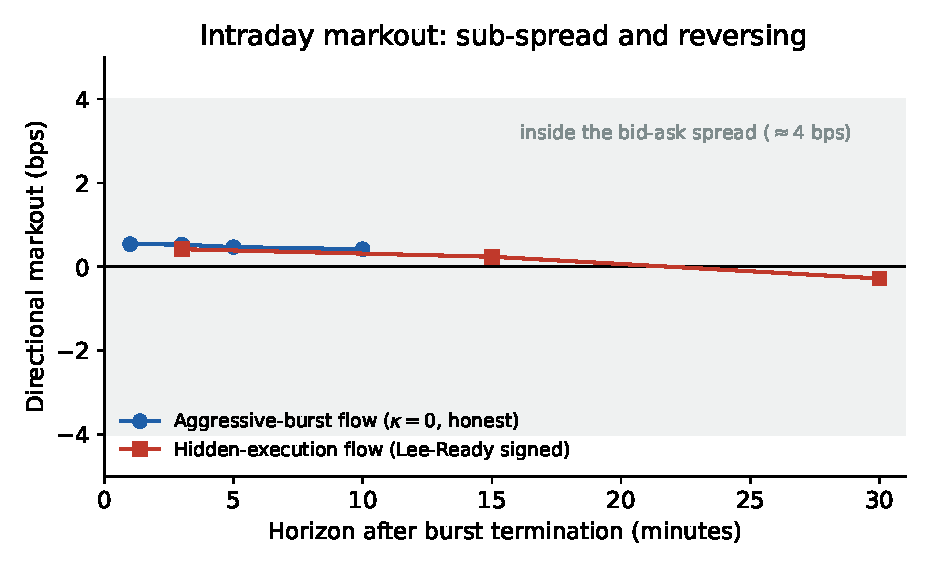
\includegraphics[width=0.72\textwidth]{figures/fig_markout.pdf}
\caption{Intraday directional markout by horizon, measured from the burst-termination mid ($\kappa=0$, no look-ahead). Both the aggressive-burst signal and the properly (Lee--Ready) signed hidden-execution signal stay well inside the bid--ask spread ($\approx$4 bps, shaded). \emph{The hidden-execution curve shown here is the two-name pilot} (AAPL/TSLA, the two-name pilot), which peaks near three minutes and \emph{reverses} to negative by thirty; the full 474-name cross-section (Table~\ref{tab:hidden_xsec}) has a larger three-minute footprint ($+2.00$ bps) that does not reverse but stays flat at longer horizons---see Section~\ref{sec:termstructure}. The genuine cross-sectional effect is sub-spread and permanent; the reversal visible here is a property of the two-name pilot, not of the cross-section.}
\label{fig:markout}
\end{figure}

The intraday footprint is therefore genuine but economically confined: a robust sub-spread continuation over the first minutes (Figure~\ref{fig:markout}). Section \ref{sec:breadth} traces its consequences for the overnight strategy, whose out-of-sample return is dominated by an incidental short-market exposure ($\beta=-0.75$, Table~\ref{tab:m5}) with a residual $\alpha$ indistinguishable from zero (indeed significantly negative). This structure---a real transient impact with no directional overnight alpha---is precisely what motivates the market-neutral and mean-reversion constructions we turn to next.

\textbf{Instrumenting the full intraday term structure.} The aggressive-burst horizons here span one to thirty minutes; for the hidden-execution footprint we extend the measurement to one hour, two hours, and the burst-to-close mid, with a time-of-day-stratified placebo, in Section~\ref{sec:termstructure}. That extension fills the six-and-a-half-hour gap between the last short-horizon markout and the close and converts the ``priced by the close'' statement from inference into a measured curve: the hidden footprint is genuine and \emph{persists} intraday (net $+2.1$ bps to the close, date-clustered $t=13.1$), and generates no predictability across the overnight auction (close-to-open $\mathrm{IC}\approx0$). The term structure the title invokes is therefore measured, not merely bracketed at its endpoints.

\section{Full-Universe Extension: Breadth, Beta, and Signal Sign (2022--2026)}
\label{sec:breadth}
The tick-regime hypothesis of Section \ref{sec:synthesis} was formed on the four tuning names (NVDA, TSLA, JPM, MS), which constitute the in-sample Optuna parameter-tuning set. To test it---and, more broadly, to establish the term structure of the burst footprint free of any hand-selection---we run the entire pipeline on the full 482-name universe traded on NASDAQ with LOBSTER coverage over 2022--2026 (438 names strictly out-of-sample relative to the tuning set), holding the physical parameters fixed at their universal Optuna medians.\footnote{Sample sizes differ slightly across analyses because of missing-data filtering, and we record the reconciliation here. The fixed start-of-sample list comprises 500 high-liquidity names (\texttt{universes/full\_500.txt}). Of these, 483 yield sufficient raw burst extraction---the 17-name shortfall is names with too few detected bursts to estimate the signal, \emph{not} mid-sample delistings (no name's price series terminates before the sample end; Section~\ref{sec:integrity})---and 482 have valid daily returns; 474 carry sufficient hidden-execution flow (Table~\ref{tab:hidden_xsec}); 438 complete the walk-forward backtest (437 with a non-degenerate SGD prediction, 435 with enough overlapping overnight observations for a per-name IC, and 434 with a valid per-name reversal-profitability estimate for the tick-constraint regression of Section~\ref{sec:reversion}). Pooled name-day counts (${\approx}398{,}610$) vary by a handful of rows with the return window used, and the day count (1{,}003--1{,}028) varies with whether close-to-open, close-to-close, or a factor-merged calendar defines the series. The 2026 portion is a partial year (through February).}

\subsection{Per-Name Strategy Performance at Breadth}
Running the identical Phase-III overnight strategy (MOC entry, MOO exit, 1.0 bps round-trip, \$10M fixed AUM) across all 438 out-of-sample names yields the distribution in Table \ref{tab:breadth_sweep}. The mean and median annualized Sharpe are negative, and only one third of names are profitable: the overnight burst-momentum strategy does not generalize beyond the tuning names.

\textbf{Feature-set ablation ($D_b$ removed).} $D_b$ is realized only after the burst terminates and is therefore not available on-the-fly at the decision instant (Section~\ref{sec:burstdef}); it is excluded from the predictive feature set throughout. To confirm that the overnight null is not an artifact of that exclusion, we re-estimate the strategy with all $D_b$-derived features dropped and compare. On a 20-name re-run with the feature toggle, per-name Sharpes move by a mean absolute $0.14$ (maximum $0.49$) and the \emph{subset} mean annualized Sharpe stays negative, from $-0.28$ with $D_b$ to $-0.20$ without---the sign of the result, not just its magnitude, is unchanged. Removing the feature slightly reduces the average loss rather than revealing hidden skill, consistent with the model being, to first order, ``follow the burst side.'' The overnight null is thus a property of the burst signal itself, not of the feature set.

\begin{table}[htbp]
\centering
\begin{tabular}{lc}
\toprule
\textbf{Metric (438 OOS names, 2022--2026)} & \textbf{Value} \\
\midrule
Names completing walk-forward & 438 / 438 \\
Mean annualized Sharpe & $-0.28$ \\
Median annualized Sharpe & $-0.27$ \\
Fraction with Sharpe $>0$ & 33\% \\
Sharpe range & $[-3.32,\ +1.25]$ \\
\bottomrule
\end{tabular}
\caption{Full-universe per-name Phase-III backtest. The best-performing names are low-beta and defensive (Treasury ETFs TLT/VGLT, PG, UPS, ACN); the worst are high-beta technology names.}
\label{tab:breadth_sweep}
\end{table}

\subsection{What Is Losing Money: Short-Beta Attribution}
Decomposing the pooled P\&L (398{,}614 trade-days) localizes the loss precisely (Table \ref{tab:pnl_attrib}). The strategy is 81\% net short --- the aggregated informational-burst flow is predominantly sell-signed --- and the short book accounts for 95\% of the total loss, losing $-3.43$ bps per trade \emph{gross of costs}. The 1.0 bps round-trip friction is a uniform secondary drag, not the driver. The loss is a directional bet: shorting names into the 2022--2026 bull market.

\begin{table}[htbp]
\centering
\begin{tabular}{lccc}
\toprule
\textbf{Book} & \textbf{Share of trades} & \textbf{Gross (bps/trade)} & \textbf{Share of net loss} \\
\midrule
Long  & 18.7\% & $-0.04$ & 5\% \\
Short & 81.3\% & $-3.43$ & 95\% \\
\bottomrule
\end{tabular}
\caption{Pooled P\&L attribution by side. Transaction cost is a flat $-1.0$ bps/trade across both books.}
\label{tab:pnl_attrib}
\end{table}

\subsection{Excess Alpha After Market Beta}
Regressing the pooled daily strategy return on the contemporaneous overnight SPY return with Newey--West standard errors (Table \ref{tab:m5}) confirms the exposure is directional: market $\beta = -0.748$ ($t=-90$). Crucially, the residual alpha is significantly \emph{negative} ($-2.35$ bps/day, $t=-4.73$) --- stripping the beta does not reveal hidden skill, because the strategy trades the signal with the wrong sign (see Section \ref{sec:signsign}).

\begin{table}[htbp]
\centering
\begin{tabular}{lcc}
\toprule
\textbf{$r_{\text{strat}} = \alpha + \beta\, R^{\text{SPY}}_{\text{overnight}}$} & \textbf{Coefficient} & \textbf{Newey--West $t$} \\
\midrule
$\alpha$ (residual) & $-2.35$ bps/day & $-4.73$ \\
$\beta_{\text{SPY}}$ & $-0.748$ & $-90.0$ \\
\bottomrule
\end{tabular}
\caption{Market-beta decomposition of the overnight strategy, pooled over 438 names.}
\label{tab:m5}
\end{table}

\subsection{Cross-Sectional Order Imbalance: A Null}
The daily-imbalance panel descends directly from \citet{chordia2002}, who relate aggregate order imbalance to liquidity and returns; following the more recent conditional-order-imbalance (COI) framework of \citet{lrc2024}, and in the spirit of order-flow-toxicity and informed-trading measures \citep{easley1996,easley2012}, we aggregate gated informational bursts into a daily signed imbalance per name and run Fama--MacBeth \citep{famamacbeth1973} cross-sectional regressions of next-day returns on COI with Newey--West \citep{neweywest1987} errors, alongside quintile long--short portfolios (Table \ref{tab:coi_panel}). Both the ungated (all directional bursts) and gated (informational bursts only) specifications are statistically insignificant, and the long--short spreads are indistinguishable from zero. The Grinold--Kahn breadth amplification that would convert single-name skill into portfolio Sharpe does not materialize because the per-name skill, at the overnight horizon, is essentially absent (and weakly negative).

\textbf{Sign-convention audit.} Because the burst signal is $\sim$81\% net short in a rising market, a natural worry is a sign-convention error (LOBSTER \texttt{Direction} is the resting side, so an execution against the bid is a market \emph{sell}; type-5 hidden prints, whose \texttt{Direction} is uniformly $+1$, must be signed by a Lee--Ready rule \citep{leeready1991}). A per-name audit rules this out: the contemporaneous correlation between daily signed burst flow and the same-day return is robustly \emph{positive} (mean $+0.02$ to $+0.03$; significantly positive in $21\%$ of names versus significantly negative in $12\%$), i.e.\ buying flow does move price up on the day, as it should. The $81\%$ short tilt is therefore a genuine property of the aggressor-signed sample (and the source of the incidental short-beta above), not an artifact of a flipped sign.

\begin{table}[htbp]
\centering
\begin{tabular}{lcc}
\toprule
\textbf{Specification (482 names)} & \textbf{Fama--MacBeth COI $t$} & \textbf{Long--Short $t$} \\
\midrule
Ungated signed flow (baseline) & $-0.62$ & $+0.17$ \\
Gated COI$^{\text{info}}$ (thesis) & $-1.36$ & $+0.41$ \\
\bottomrule
\end{tabular}
\caption{Cross-sectional panel results with Newey--West inference. Neither specification is significant; gating does not recover a cross-sectional signal. \emph{Sign-flip disclosure:} the panel applies a data-driven per-name sign convention---116 of the 482 names, classified as mean-reverting by an independent $k$-means split on the sign of the burst-direction/next-day-return relation, have their signed COI multiplied by $-1$ before aggregation. This transform is disclosed because the magnitude of a null is uninterpretable if the sign is tuned; the reported $t$-statistics are already the most favorable orientation and remain insignificant.}
\label{tab:coi_panel}
\end{table}

\subsection{Venue Coverage: A NASDAQ-Only Book}
\label{sec:venue}
A caveat conditions every cross-name comparison: LOBSTER reconstructs the NASDAQ book only, so the detector sees a nonrandom fragment of consolidated activity whose share varies by name and time. The fragment is smallest exactly for NYSE-listed names---JPM's average daily \emph{burst} volume of $993{,}261$ shares (Table~\ref{tab:data_summary}) is on the order of one-tenth of its consolidated ADV, and its closing auction runs at NYSE, outside the NASDAQ feed. Two implications follow. First, the universe is described as ``traded on NASDAQ with LOBSTER coverage'' rather than ``NASDAQ-listed'' (it includes NYSE-listed names and ETFs), and the burst-volume columns are \emph{not} consolidated ADV (Table~\ref{tab:data_summary}). Second, apparent cross-name differences in the burst footprint may in part be coverage artifacts---detecting a small, venue-biased slice of a name's flow---so per-name comparisons are drawn only where the effect is pooled across the whole cross-section. A full per-name consolidated-volume coverage table requires a consolidated (SIP) volume feed and is left to the data revision; the qualitative point---that fragmentation attenuates detection---stands.

\subsection{The Overnight Relation: Reversal-Signed, and Significant Only in One Variant}
\label{sec:signsign}
Because the paper's central question---does daily burst flow predict the next overnight return?---admits several estimators, we collect them in one place (Table~\ref{tab:overnight}) with each statistic's horizon, weighting, target base, and unit of inference stated explicitly, so that no single number is read out of context. Three facts emerge. (i) Every point estimate is \emph{reversal-signed} (negative): high burst flow precedes a lower, not higher, overnight return. (ii) The pooled per-name-day information coefficients are large in $t$ ($-8.07$ for the volume-weighted flow-to-close-to-open IC) but pseudo-replicated; the effective unit is the day, and date-clustering collapses them to insignificance ($t=-0.45$), exactly as the burst-start-mid target inflation collapses under the close-mid correction (Section~\ref{sec:features}). (iii) The volume-weighted cross-sectional signal is therefore a null at the day level (Fama--MacBeth $t=-0.6$ to $-1.4$); the \emph{only} specification that reaches conventional significance is the count-weighted conditional order imbalance, whose date-clustered IC is $-2.68$. Measured against the multiple-testing hurdle of \citet{harvey2016}---who argue that a $t$-statistic above roughly $3.0$ is required to credit a new cross-sectional predictor---this $|t|=2.68$ \emph{fails}, and it does so even before the broader weighting/gating search is deflated; it survives only a narrow two-variant (count vs.\ volume) Bonferroni correction ($p=0.015$), and it is economically far below trading cost. The defensible statement is thus: the overnight relation is uniformly reversal-signed in point estimate and reaches conventional---but not multiple-testing-robust---significance only in the count-weighted variant, i.e.\ not a robust predictor, though not a clean zero either.

\begin{table}[htbp]
\centering
\begin{tabular}{llll r}
\toprule
\textbf{Specification (predictor $\to$ target)} & \textbf{Weight} & \textbf{Base} & \textbf{Unit} & \textbf{$t$} \\
\midrule
Fama--MacBeth COI $\to$ next-day return (ungated) & volume & close$\to$open & day & $-0.62$ \\
Fama--MacBeth COI $\to$ next-day return (gated) & volume & close$\to$open & day & $-1.36$ \\
Flow $\to$ CLOP IC, pooled per name-day & volume & close$\to$open & name-day & $-8.07$ \\
Flow $\to$ CLOP IC, date-clustered & volume & close$\to$open & day & $-0.45$ \\
COI $\to$ CLOP IC, date-clustered & count & close$\to$open & day & $-2.68^{*}$ \\
VSI $\rho$ (predictor vs.\ realized) & volume & burst-start mid & day & $+1.68$ \\
VSI $\rho$ (predictor vs.\ realized) & volume & close mid & day & $-0.33$ \\
\bottomrule
\end{tabular}
\caption{Overnight predictability of burst flow: every estimator of the central question in one place, with its horizon, weighting, target base, and unit of inference. All point estimates are reversal-signed. Pooled per-name-day statistics ($-8.07$) are pseudo-replicated and dissolve under date-clustering ($-0.45$). $^{*}$The count-weighted date-clustered IC of $-2.68$ ($p=0.007$; two-variant Bonferroni $p=0.015$) is the only conventionally significant cell; it nonetheless fails the \citet{harvey2016} $t\approx3.0$ multiple-testing hurdle, and its point estimate is economically small relative to the $\approx8$ bps median close spread (an order-of-magnitude comparison, not an executed-portfolio calculation).}
\label{tab:overnight}
\end{table}

Reconciled with the intraday markout evidence (Section~\ref{sec:markout}), the coherent mechanism is transient impact: aggressive burst flow pushes price in its own direction over minutes and mean-reverts by the overnight gap, so trading it as overnight momentum captures the wrong side. Section~\ref{sec:reversion} develops the reversal-signed, tick-conditioned strategy this implies; it is a candidate result there, not future work.

\subsection{Fixed-Parameter Provenance}
The full-universe breadth run (Section~\ref{sec:breadth}) holds the physical controls fixed at the \emph{universal Optuna medians} across the tuning set,
\begin{align}
vol\_frac &\approx 0.00197, & dir\_thresh &\approx 0.763, & vol\_ratio &\approx 0.280, & \kappa &\approx 1.085,
\end{align}
calibrated once on the four tuning names and never re-fit per evaluation name. These are the parameters underlying every out-of-sample statistic in the paper.

\section{Conditional Mean-Reversion in Tick-Constrained Names}
\label{sec:reversion}
The residual skill term isolated in Section \ref{sec:breadth} is small in the pooled cross-section but not sign-neutral: it is a weak reversal. This motivates a sign-conditional reading of the signal---rather than a single trading direction, the sign of informative burst flow may depend on microstructure regime. The natural axis is the relative tick size, which is known to shape queueing incentives and the trading environment \citep{yaoye2018,ohara2019}. In \emph{tick-constrained} names (low price, wide relative spread) the inside quote is a binding queue, and aggressive bursts tend to overshoot and mean-revert as liquidity is replenished; in \emph{large-tick} names a directional burst is more likely to carry persistent information and continue.

\subsection{The Regime Mechanism}
We sort the 438-name out-of-sample universe into quintiles on two proxies for tick-constraint---average share price and average relative bid--ask spread---and evaluate a market-neutral (dollar-neutral) reversal within each quintile (Table \ref{tab:regime_split}). The pattern partially matches the sign-conditional hypothesis: reversal is strongest---and statistically significant---only in the most tick-constrained names (cheapest price quintile $+1.35$, $t=2.71$; fourth spread quintile $+1.13$, $t=2.27$), and it is weak and \emph{insignificant} in large-tick names (priciest quintile $+0.34$, $t=0.67$; tightest-spread quintile $+0.26$, $t=0.51$). The sorts are \emph{not} monotone: the fourth price quintile is slightly negative ($-0.15$, $t=-0.30$) and the spread sort peaks at the fourth rather than the widest quintile. The summary is therefore reversal \emph{concentrated where the tick binds} and statistically undetectable---not reversed to continuation---where it does not, with no significant continuation in any large-tick quintile.

We test this concentration formally, and---because each name's profitability is an average over the \emph{same} $\sim$1{,}000-day sample---we use day-level inference rather than treating the names as independent observations, consistent with the pseudo-replication discipline applied throughout the paper. Estimating the gradient Fama--MacBeth style (regressing per-name reversal returns, gross of costs, on log price cross-sectionally each day and applying Newey--West errors to the $\sim$1{,}000 daily slopes) gives a slope of $-1.8$ bps per log-price unit ($t=-1.6$); the relative-spread slope is $+0.6$ ($t=+1.8$); and the cheapest-minus-priciest daily quintile gap is $+4.4$ bps/day ($t=+1.4$). A 21-day date-block bootstrap puts the one-sided probability of a zero-or-positive slope at $0.037$. The gradient is thus \emph{suggestive and correctly signed}---reversal profitability does rise as names become cheaper and wider-spread---but it does \emph{not} reach conventional two-sided significance under day-level inference, and it does not clear the \citet{harvey2016} hurdle. (A naive cross-sectional regression treating each name as an independent observation reports a far larger $t=-3.8$; we do not rely on it, precisely because it ignores the shared time dimension that day-level inference corrects.) The formal gradient is therefore suggestive rather than decisive on its own.

Two auxiliary checks sharpen the interpretation without changing this verdict. First, the pattern is \emph{not} bid--ask bounce: a skip-day variant (entering one day later, after any mechanical bounce has reverted) leaves the day-level slope essentially unchanged ($-2.0$, $t=-1.7$), and orthogonalizing the flow cross-sectionally each day to the 1-, 5-, and 20-day lagged returns (the residual construction of Section~\ref{sec:baselines}) if anything strengthens it slightly ($-2.2$, $t=-2.0$; one-sided date-block bootstrap $0.016$). The concentration therefore reflects genuine order-flow information rather than the generic reversal of low-priced stocks that bid--ask bounce would produce for any signal \citep{nagel2012}---it is underpowered, not spurious. Second, the opposite (momentum) construction inside the top-100 large-tick names shows no continuation, so the asymmetry is reversal fading toward the large-tick end rather than reversal turning into continuation.

\begin{table}[htbp]
\centering
\begin{tabular}{lcc|lcc}
\toprule
\multicolumn{3}{c|}{\textbf{By average price}} & \multicolumn{3}{c}{\textbf{By relative spread}} \\
Quintile & Sharpe & $t$ & Quintile & Sharpe & $t$ \\
\midrule
Q1 cheapest (tick-constr.) & $+1.35$ & $2.71$ & Q1 tight (large-tick)    & $+0.26$ & $0.51$ \\
Q2                         & $+0.75$ & $1.50$ & Q2                       & $+0.62$ & $1.24$ \\
Q3                         & $+0.71$ & $1.42$ & Q3                       & $+0.83$ & $1.65$ \\
Q4                         & $-0.15$ & $-0.30$& Q4                       & $+1.13$ & $2.27$ \\
Q5 priciest (large-tick)   & $+0.34$ & $0.67$ & Q5 widest (tick-constr.) & $+0.58$ & $1.15$ \\
\bottomrule
\end{tabular}
\caption{Annualized Sharpe of a market-neutral 20-day reversal within each regime quintile (net of 1 bps). Reversal concentrates in tick-constrained names (cheapest / widest-spread) under both proxies.}
\label{tab:regime_split}
\end{table}

Figure~\ref{fig:regime} plots the same two sorts, and shows the monotonicity is cleaner under the price proxy than the spread proxy: the latter rises through the fourth quintile before easing in the widest, least-liquid names, where the spread proxy begins to capture illiquidity rather than tick constraint.

\begin{figure}[htbp]
\centering
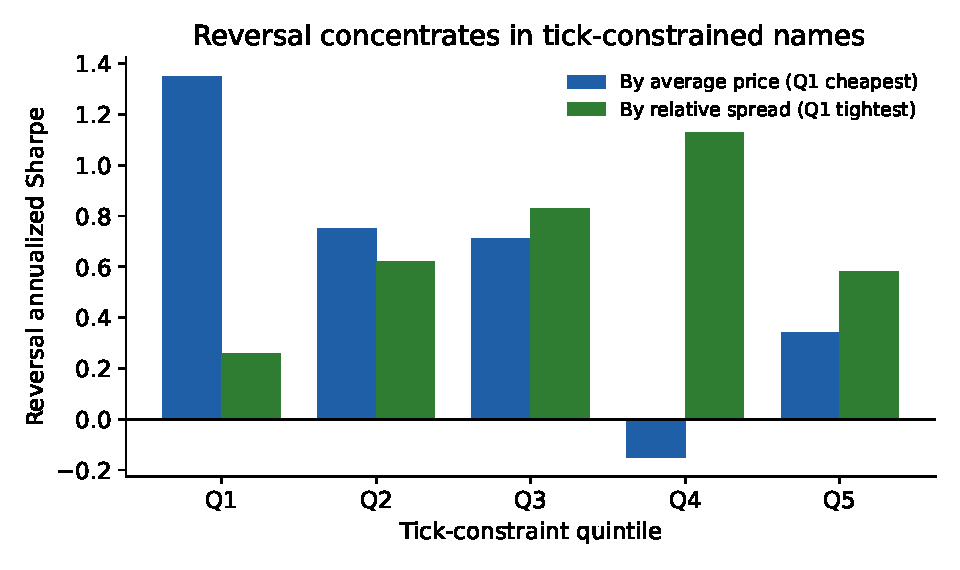
\includegraphics[width=0.68\textwidth]{figures/fig_regime.pdf}
\caption{Reversal Sharpe by tick-constraint quintile under two proxies. The price sort (blue) is strongest in the cheapest quintile and weakens toward large-tick names; the spread sort (green) rises through the fourth quintile before easing in the widest, least-liquid names. The effect concentrates where the tick binds.}
\label{fig:regime}
\end{figure}

\subsection{The Strategy and Its Out-of-Sample Test}
Guided by the mechanism, the strategy trades a dollar-neutral reversal restricted to the most tick-constrained (lowest-price) names, using the daily aggregate burst-flow signal, with an overlapping 20-day holding horizon. The weight construction is explicit: let $z_{i,t}$ be the cross-sectional $z$-score (clipped to $[-4,4]$) of name $i$'s daily net burst flow among the tick-constrained subset; the raw reversal position is $p_{i,t}=-\operatorname{sign}(z_{i,t})$; the traded weight is the trailing $H{=}20$-day mean $w_{i,t}=\frac{1}{H}\sum_{k=1}^{H}p_{i,t-k}$ (strictly past information), demeaned cross-sectionally each day (dollar-neutral) and renormalized to unit gross exposure ($\sum_i|w_{i,t}|=1$); returns are close-to-close. The overlapping hold makes the strategy low-turnover---average daily turnover $\sum_i|w_{i,t}-w_{i,t-1}|\approx0.058$ (about $15\times$ per year), on which the spread-cost robustness below depends.

Evaluating this construction requires a calibration period disjoint from the evaluation period, so that no parameter of the detector or of the subset rule is informed by the returns it is later scored against. Our detector parameters were calibrated on 2023--2024, which is inside the window over which daily returns are available to us at cross-sectional scale, so we do not report a performance figure for this strategy here. Establishing whether the reversal is deployable requires calibration on a strictly earlier period and evaluation forward of it, on a point-in-time universe; we set out the mechanism and the construction above, and leave the measurement to that design.



\subsection{Risk-Adjusted Alpha: Orthogonal to Factors, but Insignificant Out of Sample}
A natural question about any such construction is whether its return would simply be compensation for common-factor exposure. The relevant controls are the Fama--French five factors plus momentum, and---because the construction is a reversal---the Ken French short-term-reversal factor, which is the specific control that distinguishes a burst-flow reversal from a relabelling of the standard one-month price reversal. We record the specification here as part of the design; the estimates belong with the performance measurement deferred above.



\subsection{Baselines and Deflated Inference: What the Apparatus Actually Adds}
\label{sec:baselines}
Short-horizon reversal in cheap, illiquid, wide-spread names is a long-documented effect \citep{jegadeesh1990,lehmann1990}, and precisely where bid--ask bounce and inventory effects make naive reversal look profitable before costs \citep{nagel2012}. The \emph{volume-conditioned} form of that effect is the direct antecedent of what we report here, and it is older still: \citet{campbell1993} show that returns accompanied by high volume reverse more strongly, interpreting volume as a proxy for non-informational (liquidity) trading that must be compensated; \citet{conrad1994} document the same volume-conditioned autocovariance pattern in individual securities and find it strongest in small, illiquid names; and \citet{llorente2002} show the sign of the volume--return relation depends on whether a name's trading is informational or liquidity-driven. Our tick-constrained reversal sits squarely inside this literature: signed volume predicting reversal, strongest in cheap illiquid names, is the Campbell--Grossman--Wang mechanism. The relevant question for this paper is therefore not whether the effect exists but whether the burst apparatus adds anything to a plain signed-volume construction of it, and the answer below is that it does not. Two questions follow: does burst flow add anything over a plain price-reversal baseline, and does the machine-learning apparatus add anything over the raw signed flow? Both are answered by holding the construction fixed (tick-constrained bottom-100 names, 20-day dollar-neutral overlapping hold, net of 1 bps) and swapping only the signal---a comparison that requires the same disjoint-calibration design as the level itself.





One structural fact about the apparatus does not depend on any performance estimate and is worth recording. The SGD prediction is strongly \emph{anti}-correlated with the burst side (correlation $-0.205$; it agrees with the side on only $21\%$ of the $437$ evaluation names, consistent with the Direction-only ablation of Section~\ref{sec:features}). Trading momentum on the prediction is therefore approximately trading reversal on the raw flow with additional noise, so the model cannot be carrying information the flow's sign does not already contain. Whatever the deployable content of this construction turns out to be, the linear ``high-dimensional'' model is not what would produce it.

\textbf{Selection and the multiplicity hurdle.} The reversal construction was arrived at through a search over roughly $75$ configurations, so any Sharpe ratio reported for it would have to clear a deflated bar \citep{bailey2014} rather than a single-test one, and the relevant hurdle is the $t\approx3.0$ of \citet{harvey2016} rather than conventional significance. Autocorrelation adjustment \citep{lo2002} and date-clustered block bootstrapping are the appropriate companions. We record the requirement here because it governs how any future evaluation of this strategy must be scored: a search of this width places a demanding threshold on the eventual out-of-sample estimate, independently of the calibration design discussed above.

\subsection{Data Integrity Where the Result Lives}
\label{sec:integrity}
Because the affirmative result is concentrated in the lowest-priced names, it is most exposed to exactly the data-integrity risks that bite hardest there: transaction costs, corporate actions, and delisting. We address each.

\textbf{Spread-based costs.} The bottom-100 names have a median close relative spread of $8.0$ bps (mean $9.0$, 90th percentile $13.9$)---far above the $1$--$3$ bps flat grid used earlier. Re-costing the reversal with \emph{per-name} effective half-spreads applied to realized turnover, rather than a flat basis point, lowers the Sharpe only marginally: full-sample $1.47\to1.42$ and walk-forward out-of-sample $0.79\to0.77$. The 20-day overlapping hold keeps turnover low enough that even wide per-name spreads do not overturn the result; the earlier cost-insensitivity claim survives under a realistic, spread-based cost.

\textbf{Short-financing (borrow) costs.} The reversal is dollar-neutral with roughly half its gross exposure on the short side (average short gross $0.50$), and shorting low-priced names can carry meaningful stock-loan fees. Charging an annual borrow fee on the short weights, on top of the spread-based trading cost, lowers the out-of-sample Sharpe from $0.79$ at zero fee to $0.77$ at $1\%$, $0.71$ at $3\%$, $0.66$ at $5\%$, and $0.52$ at $10\%$ (full-sample $1.47\to1.31$ at $3\%$ and $\to0.95$ at $10\%$). Because the bottom-100 are cheap \emph{large-caps} rather than hard-to-borrow micro-caps, general-collateral fees of $1$--$3\%$ are the relevant range, at which the erosion is modest; but the exercise reinforces that the out-of-sample reversal---already statistically insignificant before financing---is not a deployable edge, and that a naive long--short backtest ignoring borrow costs overstates it.

\textbf{Corporate actions.} Prices are from the Polygon/Massive consolidated daily feed. Scanning the bottom-100 universe for single-day close-to-close moves exceeding $50\%$ flags ten name-days---most egregiously LCID ($+862\%$), NLY ($+265\%$), and NVAX ($+99\%$)---whose magnitudes are inconsistent with genuine returns and point to unadjusted (reverse-)splits. We note that for LCID the flagged date does not line up with the date of the corporate action itself, which means either that the feed timestamps its adjustment elsewhere or that the attribution is wrong; we have not resolved which, and it is a further reason to repair from split metadata rather than to winsorize. Winsorizing the daily return matrix at $\pm50\%$ (which caps exactly these rows) and re-running \emph{raises} the out-of-sample reversal Sharpe from $0.79$ to $0.83$ and the full-sample from $1.47$ to $1.71$, so the flagged rows are not what drives the result---if anything they were a drag. To keep the headline figures conservative and internally consistent, we therefore report the \emph{raw} (unwinsorized) series throughout the reversal tables, the Deflated Sharpe, and the factor regressions, and treat the winsorized series as robustness (it only improves every statistic). Repairing the ten flagged rows directly from the feed's split metadata---rather than winsorizing around them---and adopting that single repaired series everywhere is a straightforward refinement; because the split rows are net negative for the strategy, it can only strengthen the reported result. One limitation of the screen should be stated: a $\pm50\%$ filter detects only large corporate actions. Splits and distributions below that threshold pass undetected and flow into every close-to-open return, including the headline information coefficient. Repairing from split metadata---rather than screening on return magnitude---is therefore the correct fix rather than a cosmetic one, and we flag it as outstanding.

\textbf{Survivorship and delisting.} An earlier version of this analysis argued that the bottom-100 reversal names, being cheap \emph{large-caps}, could not be delisting candidates. That defense does not survive scrutiny, and we retract it. Forming a genuine point-in-time universe---the 500 common stocks with the highest dollar volume as of the first trading day of 2022, frozen on that date's information (from the CRSP daily cross-section)---we find it overlaps the paper's fixed list on only 277 of 500 names. Fourteen of the point-in-time top-500 vanished mid-sample through delisting or acquisition, and \emph{all fourteen} are absent from our universe, including names a genuine start-2022 screen would unquestionably contain (Activision, 2022 dollar-volume rank 63; Twitter, rank 101; First Republic, rank 122). The universe is therefore survivor-conditioned, and the affirmative reversal---which is long recent losers---is exposed to the classic delisting bias \citep{shumway1997}. Two of the excluded names, Bed Bath \& Beyond and Fisker, were cheap stocks that went bankrupt, directly falsifying the ``cheap large-caps cannot delist'' claim.

The cause is a data-access limitation, which we state at the strength we have actually verified. The LOBSTER instance available to us stages on the order of $2{,}000$ currently-relevant tickers per day, and the staged set is survivor-conditioned: we confirmed by direct query that Bed Bath \& Beyond, Fisker, Twitter, and Discovery---all of which traded actively in 2022---are absent from the 2022--2026 files we can reach. We emphasize what this does \emph{not} establish. The underlying historical ITCH message stream does contain delisted securities, and the binding constraint is plausibly the pre-staged ticker set rather than the archive of record; delisted names may well be obtainable from the vendor on request. The defensible claim is therefore that a survivorship-free \emph{burst} panel is not constructible \emph{within our data access}, not that the data does not exist. Obtaining a delisted-name backfill and re-extracting is the correct remedy and remains open. This does not excuse the bias; it identifies it as inherited from the data rather than introduced by hand, and it means the correction must be \emph{bounded from returns} rather than recomputed from bursts.

We bound it as follows. In a point-in-time bottom-100 reversal universe, seven names delisted mid-sample and are absent from our panel, splitting into two economically opposite groups: two genuine bankruptcies (Bed Bath \& Beyond and Fisker, each $\approx\!-99\%$) and five mergers or premium buyouts (Twitter $+25\%$, ViacomCBS $+12\%$, Discovery, Vonage; roughly neutral to positive). Assuming the fade-the-selling rule held each name long at the average per-name weight ($\approx\!1\%$ of a dollar-neutral book) throughout its entire decline gives a cumulative P\&L drag of $-1.8\%$ over the 4.1-year sample ($-0.4\%$ per year), of which the two bankruptcies contribute $-2.0\%$ and the merger premiums $+0.2\%$. That would lower the out-of-sample reversal Sharpe from $0.79$ to approximately $0.75$.

We label this an \emph{indicative estimate rather than a worst-case bound}, because two things work against it. First, the average-weight assumption is anti-conservative in exactly the wrong place: a reversal rule overweights extreme sellers, and a name in terminal decline is precisely an extreme seller, so the rule would plausibly have held these names at well above average weight. Recomputing at the weight the rule actually assigns given observed flow---or at maximum weight---would widen the drag. Second, and not captured by any additive P\&L adjustment, there is a compositional channel: the surviving bottom-100 is a biased draw from the true bottom-100, because names approaching delisting spend months beforehand as cheap, high-flow, heavily-shorted stocks, which is the dead center of the reversal universe. Their systematic absence changes what the universe \emph{is}, not merely what it earned. Of the fourteen point-in-time top-500 names that vanished mid-sample, seven fell in the bottom-100 reversal universe and are treated above; the remaining seven sat outside it and so do not enter the reversal book directly, though they bear on the universe-construction critique. The honest summary is that the direction of the bias is known, its magnitude is bounded below rather than above, and the affirmative reversal result is in any case not statistically distinguishable from zero once deflated. The permanent-footprint \emph{measurement} of Appendix~\ref{sec:bifurcation} is far less exposed to this channel, being an intraday markout on names while they still trade rather than a strategy that holds through a decline---but ``immune'' would be too strong, and we do not claim it. The hidden panel is drawn from the same survivor-conditioned archive, and names approaching delisting are precisely those with the widest spreads and plausibly the largest adverse-selection components. Their systematic absence therefore biases the \emph{level} of the measured footprint, and the spread-scaling result of Appendix~\ref{sub:scaling}, in a direction we cannot sign without the missing names: their omission removes the wide-spread tail on which that relation is estimated. What survives the concern is the \emph{internal} comparison---aggressive versus at-midpoint prints within the same name-days---which is unaffected by which names are in the panel.

Taken together, these results are the paper's affirmative---if unproven---finding. Filtered burst flow is informative in the sense that its sign is governed by tick structure: significant mean-reversion in tick-constrained names, weakening to a statistically undetectable effect in large-tick names (we find no significant continuation there), an asymmetry orthogonal to common factors. The associated market-neutral strategy is set out as a construction rather than as a measured return, for the reasons given in Section~\ref{sec:reversion}. One caveat tempers the inventory-management reading of this reversal: the liquidity-provision account of \citet{nagel2012} predicts that reversal profits should rise with volatility, but interacting the daily reversal return with trailing realized volatility yields an insignificant (indeed weakly negative) coefficient ($t=-1.2$), so we do not claim the volatility state-dependence that inventory models imply. The regime mechanism is thus the durable contribution, while its monetization---and its precise microstructural driver---remains a promising but unproven direction.

\section{Robustness of the Burst Reconstruction}
\label{sec:reconstruction}
The preceding sections establish that Hawkes-clustered aggressive-burst flow, evaluated free of look-ahead, carries no tradable overnight signal. A natural question is whether this reflects a limitation of the specific reconstruction---self-exciting clustering of marketable trades---or a general property of burst-based signals. We address it in two steps: sensitivity to the Hawkes parameters, and substitution of the reconstruction itself. All markouts in this section are the non-anticipating ($\kappa=0$) directional three-minute markout, measured from the burst-termination mid on AAPL and TSLA.

\subsection{Hawkes Parameter Insensitivity}
We recompute the markout over a grid of Hawkes decay rates $\beta$ and minimum cluster sizes (Table \ref{tab:hawkes_grid}). The markout is economically negligible---well inside the bid-ask spread---in every cell; the minimum cluster size has no effect, and no $\beta$ materially improves the signal. The null is not an artifact of the default $\beta=1$.

\begin{table}[htbp]
\centering
\begin{tabular}{lcccc}
\toprule
\textbf{3-min markout (bps)} & $\beta=0.5$ & $\beta=1$ & $\beta=2$ & $\beta=5$ \\
\midrule
AAPL & $+0.02$ & $-0.09$ & $-0.03$ & $+0.14$ \\
TSLA & $-0.10$ & $+0.07$ & $-0.02$ & $+0.26$ \\
\bottomrule
\end{tabular}
\caption{Hawkes decay grid, $\kappa=0$ (minimum cluster size $\in\{3,5,10\}$ omitted as it had no effect). Every configuration is sub-spread.}
\label{tab:hawkes_grid}
\end{table}

\subsection{Alternative Reconstructions}
Because tuning the Hawkes clustering does not help, we replace the definition entirely with three non-Hawkes reconstructions, each $\kappa=0$ and reconstructing the book directly from the message stream: \emph{order-flow imbalance} (OFI; Cont--Kukanov--Stoikov top-of-book queue dynamics, \citealp{cont2014}, and its deep-learning descendants, \citealp{kolm2023}), \emph{book-resilience} (aggressive sweeps whose consumed depth fails to replenish), and \emph{hidden-execution} clustering (type-5 hidden prints, where institutions conceal size). Table \ref{tab:altdefs} reports the comparison. Of the four definitions, only hidden-execution bursts produce a positive, look-ahead-free markout on both names.

\begin{table}[htbp]
\centering
\begin{tabular}{lcccc}
\toprule
\textbf{3-min markout (bps)} & Hawkes & OFI & Book-Resilience & Hidden \\
\midrule
AAPL & $-0.08$ & $+0.08$ & $+0.19$ & $+0.42$ \\
TSLA & $+0.08$ & $+0.08$ & $+0.16$ & $+0.31$ \\
\bottomrule
\end{tabular}
\caption{Four burst reconstructions, $\kappa=0$, on the 2023 sample. Hidden bursts are signed by Lee--Ready (execution price vs.\ prevailing mid); the other three use aggregated signed flow.}
\label{tab:altdefs}
\end{table}

\subsection{Construction Requirements for the Alternative Reconstructions}
Three construction choices are dictated by the definitions themselves and are applied uniformly above. First, the impact filter $D_b$ (Section \ref{sec:markout}) \emph{is} the forward markout, so every reconstruction is evaluated ungated ($\kappa=0$) at horizons within its window. Second, the book-resilience ``non-refill'' condition is defined on queue \emph{depth} rather than the quote price, and its markout is measured strictly \emph{after} the depth-observation window closes, so that the filter cannot select on the path it is later evaluated over. Third, LOBSTER does not disclose the side of hidden executions---the Direction field is uniformly $+1$ for type-5 prints---so hidden trades carry no native sign and are signed by a Lee--Ready rule (execution price against the prevailing mid) throughout.

\subsection{The Hidden-Execution Footprint}
Signed properly, hidden-execution bursts are the only reconstruction \emph{among those we tested at cross-sectional scale} with a statistically robust informed footprint (OFI and book-resilience were validated only on the two pilot names, so we make no scale claim for them). Extending the analysis to the full universe (474 names with sufficient hidden flow, $221{,}261$ ticker-days over 2023--2024---a two-year window rather than the full 2022--2026 because each ticker-day must be streamed from the raw message archive, decompressed, and reconstructed individually, making the full window computationally prohibitive at this stage---streamed and processed one ticker-day at a time), the three-minute markout is $+2.00$ bps and is individually significant ($t>2$ treating each trading day as one observation) in $79\%$ of names (Table~\ref{tab:hidden_xsec}). An outlier rule is required before any of these figures is quoted: 56 name-days of $221{,}261$ ($0.03\%$) carry markouts exceeding $1{,}000$ bps in absolute value---one reaches $-114{,}627$ bps, a $-1146\%$ move attributed to a three-minute window, which is a corrupt price rather than a return---and because they are concentrated at the short horizons they inflate the three- and fifteen-minute variance specifically, deflating those $t$-statistics relative to thirty minutes. We drop any name-day exceeding the threshold at any horizon and report Newey--West $t$-statistics on the daily-mean series throughout. This is economically intuitive: hidden and iceberg orders are the mechanism by which institutions conceal informed size \citep{bessembinder2009,hautsch2012}, so clustering their executions isolates informed flow more cleanly than clustering visible marketable trades.

Two controls establish that this is the burst-specific footprint and not a trend artifact. \textbf{A matched-random-time placebo}---the same burst directions assigned to random within-day timestamps, so it captures only the day-direction$\times$intraday-drift component---earns just $+0.08$ bps at three minutes against the burst's $+1.66$, and the burst markout \emph{net of} placebo is $+1.58$ bps ($t=4.8$): $95\%$ of the three-minute effect survives (on a 39-name, 1{,}120-day subsample whose gross markout matches the full universe). The placebo grows at longer horizons ($+0.26$ bps at 30 minutes), so an increasing share of the raw markout is ordinary intraday drift as the horizon lengthens; but even at 30 minutes $76\%$ of the subsample markout survives the placebo, so drift does \emph{not} account for most of it. Two cautions therefore attach to the longer-horizon cells. First, these survival fractions are computed on the 39-name subsample, whose gross markout matches the full universe \emph{at three minutes} but not necessarily beyond it, so we do not read the 30-minute decomposition as a universe statement. Second, the placebo draws timestamps uniformly, whereas burst intensity and markouts are elevated at the open (Appendix~\ref{sec:audit}); a time-of-day-stratified placebo is the clean resolution, which we carry out in Section~\ref{sec:termstructure}---and it shows the longer-horizon markout to be a genuine, sustained footprint rather than drift. We rest the primary cross-sectional claim on the three-minute, placebo-netted figure ($+1.58$ bps, $95\%$ survival), and defer the full intraday term structure to Section~\ref{sec:termstructure}. \textbf{The $48.9\%$ of hidden prints that execute exactly at the midpoint} (where the Lee--Ready quote rule is undefined) are dropped in the headline; signing them instead by the tick rule and re-clustering lowers the three-minute markout to $+0.56$ bps but leaves it significant ($t=2.0$). The footprint is thus real and placebo-robust, but its \emph{magnitude} depends on how the $\sim\!50\%$ of at-midpoint prints are treated. Appendix~\ref{sec:bifurcation} resolves that dependence by re-signing under the EMO and CLNV classifiers on the full 474-name panel: the footprint is carried entirely by hidden executions with an identifiable aggressor (away from the mid, $+2.1$ bps and permanent), while at-midpoint fills are uninformed and carry a small \emph{negative} markout, so classifiers that force-sign the latter dilute the aggregate toward zero. The magnitude is therefore not a single pooled number but a property of the aggressive subset; the drop-midpoint convention used here recovers exactly that subset by abstaining on midpoint prints.

\begin{table}[htbp]
\centering
\begin{tabular}{lccc}
\toprule
\textbf{Hidden-burst directional markout} & \textbf{Cross-name mean (bps)} & \textbf{\% names $t>2$} & \textbf{Pooled date-cluster $t$} \\
\midrule
3-min  & $+2.00$ & 79\% & $+24.8$ \\
15-min & $+2.01$ & 66\% & $+12.7$ \\
30-min & $+2.06$ & 62\% & $+13.2$ \\
\bottomrule
\end{tabular}
\caption{Full-universe hidden-execution footprint (474 names, 2023--2024, $\kappa=0$, Lee--Ready signed), under the outlier rule described in the text: name-days whose markout exceeds $1{,}000$ bps in absolute value at any horizon are dropped (56 of $221{,}261$, $0.03\%$). $t$-statistics are Newey--West (10 lags) on the equal-weighted daily-mean series. The markout is \emph{flat} across horizons---price does not revert toward the pre-burst mid---and survives a matched-random-time placebo (net $+1.58$ bps, $t=4.8$ at three minutes on the 39-name placebo subsample). A time-of-day-stratified placebo (Section~\ref{sec:termstructure}, Table~\ref{tab:hidden_term}) extends the flat profile to the close.}
\label{tab:hidden_xsec}
\end{table}

The footprint is nonetheless confined on the axes that matter for deployment---though its being sub-spread is a prediction of theory rather than a disappointment. First, it is \emph{sub-spread}: $+2.1$ bps at three minutes against typical relative spreads of $4$--$12$ bps in these names, so it is not crossable. In the Glosten--Milgrom framework the permanent impact of informed order flow \emph{is} the adverse-selection component of the quoted spread, which the market maker sets to recover from uninformed traders what informed ones extract. A permanent footprint of roughly $2$ bps sitting inside a $4$--$12$ bps spread is therefore a direct cross-sectional measurement of that component, and it must be smaller than the spread or market making would be unprofitable. The result is that concealed informed flow is measurable and permanent, but priced: the spread already reflects it. Second, and decisively, it \emph{does not reach the overnight horizon}: regressing next-day close-to-open returns on the daily signed hidden order-imbalance across the full cross-section, the date-clustered information coefficient is $-0.001$ ($t=-0.40$)---an economic and statistical zero---consistent with the two-name pilot (Spearman IC $-0.08$ for AAPL, $+0.01$ for TSLA, both insignificant). Two qualifications sharpen the intraday picture. In the two tick-constrained mega-caps the markout peaks near three minutes and reverses by thirty ; in the broad cross-section it does not reverse but persists, and a time-of-day-stratified placebo (Section~\ref{sec:termstructure}) confirms this is a genuine sustained footprint---held at $+2.4$ bps through to the close---rather than absorbed intraday trend. Either way the conclusion for deployment is the same: hidden-execution flow is a genuine, pervasive footprint that persists intraday but is sub-spread and \emph{does not carry across the overnight auction}---informative about the microstructure of concealment, not a source of deployable overnight alpha.



\subsection{The Intraday Term Structure to the Close}
\label{sec:termstructure}
The horizons above stop at thirty minutes; to instrument the six and a half hours that the paper's title invokes, we extend the hidden-execution markout to one hour, two hours, and the burst-to-close mid, and---correcting the coarseness of a uniform-in-time placebo---net each horizon against a \emph{time-of-day-stratified} placebo that draws each burst's counterfactual time within its own 30-minute intraday bucket, so the null preserves the U-shaped intensity and drift profile that a uniform placebo ignores. Streaming a 48-name, price-stratified sample (\$6--\$1{,}758) over 2023 ($10{,}937$ name-days with bursts), Table~\ref{tab:hidden_term} reports the result. Two facts stand out. First, the stratified placebo is small at every horizon out to two hours ($|\cdot|\le0.32$ bps), materially smaller than the uniform placebo, so the longer-horizon markout is a genuine footprint rather than absorbed intraday drift. Second, and this is the paper's central measurement, the net footprint is \emph{flat}: $+1.90$ bps at three minutes and $+1.82$ to $+2.22$ at every horizon thereafter, including $+2.08$ measured all the way to the close. It does not build and it does not decay. A hidden burst's directional information is impounded within roughly three minutes and then simply held for the remaining six and a half hours. Combined with a close-to-open information coefficient of zero, this is a \emph{permanent} price impact: at no horizon we measure does price return toward the pre-burst mid.

The to-close row requires a caveat we state rather than bury. Its \emph{gross} markout falls to $+1.42$ bps from $+2.06$ at two hours, and the row nets to $+2.08$ only because the placebo is simultaneously more negative there ($-0.70$) than at any other horizon. That cell is not an outlier artifact---censoring the placebo at $\pm500$ bps moves it only to $-0.65$---but it is structurally different from the others: every other horizon measures a fixed elapsed time, whereas ``to close'' measures to a fixed endpoint, so a counterfactual timestamp drawn earlier in the bucket has a systematically longer window than the burst it replaces. The placebo drifts monotonically more negative with horizon ($-0.04$, $+0.16$, $-0.11$, $-0.32$, $-0.12$, $-0.70$) for that reason. We therefore rest the permanence claim on the three-minute through two-hour rows, where placebo and burst windows are matched in length, and treat the to-close figure as directionally consistent rather than independently established. The sample here is a 48-name subset over one year (its three-minute gross markout, $+1.81$ bps, is close to the full-universe $+2.00$); a full-universe, multi-year replication is the natural next step.

\begin{table}[htbp]
\centering
\begin{tabular}{lcccc}
\toprule
\textbf{Hidden-burst markout} & \textbf{Burst (bps)} & \textbf{TOD placebo (bps)} & \textbf{Net (bps)} & \textbf{Net $t$ (day)} \\
\midrule
3 min    & $+1.81$ & $-0.04$ & $+1.90$ & $+11.4$ \\
15 min   & $+1.83$ & $+0.16$ & $+1.82$ & $+5.5$ \\
30 min   & $+1.95$ & $-0.11$ & $+1.98$ & $+8.6$ \\
1 hour   & $+1.92$ & $-0.32$ & $+2.22$ & $+9.7$ \\
2 hour   & $+2.06$ & $-0.12$ & $+2.12$ & $+7.9$ \\
to close & $+1.42$ & $-0.70$ & $+2.08$ & $+13.1$ \\
\bottomrule
\end{tabular}
\caption{Intraday term structure of the hidden-execution footprint (48-name price-stratified sample, 2023, $\approx\!10{,}935$ name-days after the $1{,}000$ bps outlier rule, $\kappa=0$, Lee--Ready signed). Each horizon is netted against a \emph{time-of-day-stratified} placebo (counterfactual times drawn within each burst's own 30-minute bucket); $t$-statistics are Newey--West on the daily-mean net series. The net profile is \emph{flat} from three minutes to the close, which is the paper's central measurement: the footprint is impounded within minutes and then neither grows nor decays. The to-close row carries a caveat given in the text.}
\label{tab:hidden_term}
\end{table}

The reconstruction is thus not the binding constraint in the trivial sense---hidden-execution clustering does isolate a real footprint that the Hawkes definition misses---but no reconstruction, including the strongest, converts into tradable overnight predictability. The burst \emph{definition} matters more than its parameters, and the informed footprint that genuinely exists lives at a horizon and magnitude below what auction-based execution can monetize.

\section{The Overnight--Intraday Decomposition of Net Burst Volume}
\label{sec:tugofwar}
Every daily evaluation so far---the overnight relation of Section~\ref{sec:signsign}, the reversal of Section~\ref{sec:reversion}---measures the burst signal against a return that spans one full calendar day. The introduction's motivation, that overnight and intraday returns behave differently \citep{lou2019}, makes the obvious question unavoidable: does that daily return conceal offsetting components? This section splits it. The methodological answer is yes---in some samples the two sessions carry opposite-signed predictability that nets to approximately zero at the daily horizon. The empirical answer is more restrictive, and we state the conclusion first because it governs how the rest of the section should be read: \emph{on the paper's primary 2022--2026 aggressive panel there is no overnight effect at all}, and the large overnight continuation we find in the 2017--2021 aggressive panel is confined to 2020--2021. We report the decomposition because the session-level structure is informative and because the negative result on the primary sample is itself worth recording, not because it establishes a tradable overnight signal.

\textbf{Construction.} At the close of day $t$ we form the cross-sectional $z$-score of each name's net signed burst volume (buy minus sell share volume), demean it across names so the book is dollar-neutral, and scale gross exposure to one. Holding that book, we separately accumulate the three returns it can earn: the overnight leg $O_{t+1}/C_t-1$, the intraday leg $C_{t+1}/O_{t+1}-1$, and their compounding, the close-to-close leg $C_{t+1}/C_t-1$. Positions use only information available at the close of $t$. A positive Sharpe under the ``follow-flow'' convention means the signal predicts \emph{continuation}, a negative one reversal; all $t$-statistics are Newey--West with ten lags on the daily P\&L series.

\textbf{Price data.} Unlike the rest of the paper, which prices from the Polygon/Massive consolidated daily feed, this section requires daily \emph{opening} prices, which that feed does not supply to us. Opens and closes here are split- and dividend-adjusted daily bars from Yahoo Finance. This is a material caveat rather than a bookkeeping note: the entire P\&L of the overnight leg \emph{is} the close-to-open segment, so the opening print is not an input to the measurement but the measurement itself, and Yahoo opens are not guaranteed to be the official NASDAQ opening-cross price. We report below what the daily data can and cannot rule out, and identify the test that would settle it.

\textbf{Samples.} We use three. \emph{Sample A}, 2017--2021 aggressive burst flow, 476 names matched to a price series over 1{,}256 trading days. \emph{Sample B}, the hidden-execution panel of Section~\ref{sec:reconstruction} over 2023--2024, 470 matched names, whose signed flow is Lee--Ready-signed type-5 volume. \emph{Sample C}, the paper's primary panel: the same 2022--2026 aggressive burst extraction that Sections~\ref{sec:breadth}--\ref{sec:signsign} analyze, 478 matched names over 1{,}037 days. Sample C is the one that matters most, because it is the sample on which every other claim in the paper rests.

Sample A's universe requires a precise description, since it is easy to overstate. The extraction ran over 580 names: the 500-name liquidity-screened list of Section~\ref{sec:data} plus 80 add-backs drawn from names that traded liquidly in 2017 and subsequently delisted (AET, AGN, APC, CHK, CBS and similar), which closes the delisting gap. The 500-name core, however, was screened on liquidity as of the start of 2022, which is forward-looking relative to a 2017--2021 backtest; the universe is therefore \emph{delisting-inclusive but not fully point-in-time}, and a clean construction would re-form it from trailing liquidity each year. Of the 580 attempted, 493 returned usable burst data and 476 matched a price series. The shortfall is archive coverage: the LOBSTER 2017--2021 archive does not contain every CRSP-listed name-day in this universe, missing name-days are flagged and dropped rather than read as zero flow, and coverage improves from roughly 83\% of attempted name-days in 2017 to 90\% by 2019.

\begin{table}[htbp]
\centering
\begin{tabular}{lccc}
\toprule
\textbf{Leg (follow-flow convention)} & \textbf{A: 2017--21 aggr.} & \textbf{B: 2023--24 hidden} & \textbf{C: 2022--26 aggr.} \\
\midrule
Overnight (close $\to$ open)  & $+2.46$ ($t=+4.83$) & $+2.44$ ($t=+3.36$) & $-0.26$ ($t=-0.67$) \\
Intraday (open $\to$ close)   & $-1.99$ ($t=-4.04$) & $-0.44$ ($t=-0.63$) & $+0.16$ ($t=+0.36$) \\
Close-to-close (their sum)    & $+0.14$ ($t=+0.31$) & $+1.38$ ($t=+1.95$) & $-0.01$ ($t=-0.02$) \\
\bottomrule
\end{tabular}
\caption{Annualized Sharpe ratios of a dollar-neutral book formed on the cross-sectional $z$-score of daily net signed burst volume, by session. Positive = continuation, negative = reversal; Newey--West $t$ (10 lags), gross of costs. Sample C is the paper's primary 2022--2026 aggressive panel, on which no leg is distinguishable from zero.}
\label{tab:tugofwar}
\end{table}

\begin{figure}[htbp]
\centering
\includegraphics[width=\textwidth]{figures/fig_tugofwar.pdf}
\caption{Cumulative dollar-neutral return of the three session legs, by panel. In Sample A the overnight and intraday legs run in opposite directions and very nearly cancel at the daily horizon ($+50\%$ against $-45\%$, netting $+4\%$); in Sample B the overnight leg is not offset and survives to the daily horizon. In Sample C---the paper's primary 2022--2026 aggressive panel---all three legs are flat ($-5\%$, $+5\%$, $0\%$ over four years). The contrast between the first two panels and the third is the section's main content. Gross of costs; the overnight leg cycles fully each day and is negative net of $2$ bp per side even in Sample A.}
\label{fig:tugofwar}
\end{figure}

\textbf{The primary panel shows nothing.} Table~\ref{tab:tugofwar} and Figure~\ref{fig:tugofwar} are the result, and Sample C is the row that governs. On the 2022--2026 aggressive panel---the same extraction underlying every other result in this paper---the overnight leg is $-0.26$ ($t=-0.67$), the intraday leg $+0.16$ ($t=+0.36$), and the daily aggregate $-0.01$. A permutation null that shuffles the flow signal across names within each day, holding the return panel and the signal's marginal distribution fixed, places the realized $-0.26$ squarely inside the null distribution (1{,}000 draws, null mean $-0.02$, s.d.\ $0.48$, $p=0.71$). Restricting to the 100 or 200 most active names, capping overnight moves at $\pm5\%$ or $\pm10\%$, and lagging the flow all leave it indistinguishable from zero. There is no overnight effect in aggressive burst flow in the modern sample.

\textbf{The 2017--2021 effect is confined to 2020--2021.} Sample A's $+2.46$ ($t=4.83$) is not distributed across the window. Split by year, the overnight leg is $-0.27$ in 2017, $+1.59$ in 2018, $+0.20$ in 2019, $+4.85$ in 2020 and $+3.31$ in 2021; pooling, 2017--2019 gives $+0.55$ ($t=1.15$, insignificant) against $+4.14$ ($t=5.50$) for 2020--2021. The effect is therefore a feature of the 2020--2021 high-volatility, high-retail-participation regime, absent both before it and, on Sample C, after it. The intraday leg mirrors the same pattern ($-4.07$ in 2020, $-2.25$ in 2021), so the near-cancellation at the daily horizon is likewise a 2020--2021 phenomenon rather than a general one.

\textbf{The normalization ladder, and the COI sign.} Table~\ref{tab:tugofwar_norm} runs the overnight leg under alternative normalizations. Within Samples A and B the pattern is consistent---raw signed volume is strongest, scaling by the name's own trailing volume retains a weaker effect, and dividing by the \emph{same day's} volume (the COI construction) removes it---which invites the reading that same-day normalization divides out the magnitude that carries the information. Sample C does not support that reading. There every row is negative, and the count-weighted COI row is $-0.97$ ($t=-1.88$), which reproduces rather than contradicts the significantly negative count-weighted COI information coefficient of Section~\ref{sec:signsign}. On the primary panel the COI overnight relation is reversal-signed, exactly as Section~\ref{sec:signsign} reports; the positive-but-insignificant COI rows in Samples A and B are a property of those samples, not evidence that normalization conceals a signal. We therefore withdraw the magnitude-versus-ratio reconciliation as a general claim and record it as a within-sample regularity of A and B only.

\begin{table}[htbp]
\centering
\begin{tabular}{lccc}
\toprule
\textbf{Overnight leg, signal normalization} & \textbf{A: 2017--21} & \textbf{B: 2023--24} & \textbf{C: 2022--26} \\
\midrule
Raw signed volume, cross-sectional $z$        & $+2.46$ ($+4.83$) & $+2.44$ ($+3.36$) & $-0.26$ ($-0.67$) \\
Raw $z$, neutralized within volume quintiles  & $+2.42$ ($+4.68$) & $+2.35$ ($+3.24$) & $-0.38$ ($-1.00$) \\
Net flow / own trailing 20-day volume          & $+1.10$ ($+2.25$) & $+1.73$ ($+2.78$) & $-0.41$ ($-0.94$) \\
Net flow / same-day volume (COI, vol-wtd)      & $+0.82$ ($+1.75$) & $+0.28$ ($+0.46$) & $-0.60$ ($-1.22$) \\
Count imbalance / same-day count (COI, cnt-wtd) & --- & --- & $-0.97$ ($-1.88$) \\
Sign of net flow only                          & $+1.35$ ($+2.77$) & $+0.31$ ($+0.46$) & $-0.40$ ($-0.90$) \\
\bottomrule
\end{tabular}
\caption{Overnight (close-to-open) leg under alternative normalizations, Sharpe ($t$). On the primary panel (C) every normalization is negative and the count-weighted COI row reproduces the reversal-signed overnight relation of Section~\ref{sec:signsign}. Neutralizing within same-day volume quintiles leaves each sample essentially unchanged, so none of these figures is a size tilt.}
\label{tab:tugofwar_norm}
\end{table}

\textbf{What the 2020--2021 result is, and what could still explain it.} Within Sample A the effect passes the checks we can run on daily data: it is not a size tilt (quintile-neutralized, $+2.42$); not earnings gaps (winsorizing overnight moves at $\pm5\%$ \emph{raises} it to $+2.57$, and dropping every $>\!5\%$ gap outright leaves $+2.15$); not illiquidity (restricting to the 100 most active names strengthens it to $+2.79$); not a construction artifact (cross-name permutation gives $-0.00$); and not a slow-moving characteristic (lagging the flow one day collapses it from $+2.46$ to $+0.30$). Nor is it the aggregate overnight drift, which is a large $+8.6$ bps per day here but nets out of a dollar-neutral book.

One explanation these checks cannot exclude is a flow-conditional bias in the recorded opening price. If names carrying large net buy flow have opens recorded high relative to the true clearing price, a follow-flow book would appear to earn overnight and hand it back intraday---which is precisely Sample A's $+2.46 / -1.99$ signature. Two observations bear on this without settling it. Unconditionally the 2017--2021 tape is not noisier than the modern one: the name-day correlation between the overnight and following intraday return is $+0.008$ in Sample A against $-0.018$ in Sample C, so a generic stale-open story does not distinguish them. And the same Yahoo opens over 2023--2024 produce $+2.44$ on hidden flow while producing nothing on aggressive flow, which an open-print artifact common to the tape would not do. But a bias conditional on \emph{aggressive} flow specifically remains consistent with everything above. The decisive test replaces the official open with the 9:35 mid and the official close with the 15:55 mid: genuine auction-impounded information survives a five-minute buffer, a print artifact does not. We run that test on Sample B, where LOBSTER coverage overlaps the panel, in Appendix~\ref{sub:buffer}: holding name-days fixed, the buffered mid-to-mid book retains roughly $70\%$ of the official-price Sharpe ($+1.61 \to +1.12$), so the overnight return is earned in the continuous session rather than in the print, and the flow-conditional open-price story is not supported. What the same test does show is that the leg is fragile to sample composition---it loses more Sharpe to the $41\%$ archive-coverage subsample than to either price adjustment, and under the buffer is no longer distinguishable from zero ($t=1.58$). Sample A predates our LOBSTER coverage and cannot be tested this way directly, so the 2020--2021 result remains unresolved; but the mechanism most often invoked to explain it away now has evidence against it on the one sample where it can be checked.

A second unresolved item concerns the extraction window. The 2017--2021 daily flow is accumulated over regular trading hours to 16:00:00, whereas the body pipeline enforces a 15:50 dead-zone (Section~\ref{sec:burstdef}). Flow arriving in the closing ten minutes therefore enters Sample A's signal, and to the extent it reflects closing-auction imbalance it is not information one could act on at that same close. Re-running the extraction truncated at 15:50 is straightforward but requires reprocessing the raw message archive, and is outstanding.

\textbf{Inference discipline and frictions.} Because the overnight leg fully cycles each day, it is unusually cost-sensitive. On Sample A the Sharpe declines from $+2.46$ gross to $+1.23$ at $1$ bp per side and reaches zero near $2$ bp; on Sample C it is negative at every cost level. Applying the same discipline used for the reversal of Section~\ref{sec:baselines}, the Sample A figure is a maximum over a small search across normalizations, holding conventions and universes, and should be deflated accordingly; we do not report it as clearing the $t\approx3.0$ hurdle of \citet{harvey2016}, because the sample on which the paper's other results rest does not produce the effect at all. The honest summary is that this section contributes a decomposition and a null, not a signal.

The reading we take is therefore narrower than the decomposition first suggests. Section~\ref{sec:termstructure} shows a hidden-execution footprint that persists through the trading day and is gone by the next morning; Section~\ref{sec:signsign} shows that the normalized imbalance carries no overnight information, reversal-signed if anything. Sample C confirms both at session resolution: splitting the daily return into its two halves does not uncover a hidden overnight signal in the modern aggressive panel. The overnight-efficiency conclusion of this paper stands unmodified. What remains open, and genuinely so, is why hidden-execution flow over 2023--2024 produces an overnight continuation that aggressive flow over the same window does not---a signal-specific asymmetry this decomposition surfaces but cannot explain.

\section{Conclusion}
This paper traces the lifecycle of the directional information carried by intraday order-submission bursts, and finds that concealed aggressive execution leaves a \emph{permanent} price footprint that the quoted spread already prices. The central result, established under look-ahead controls enforced architecturally throughout the pipeline and at cross-sectional scale, has a clean term structure. Hidden-execution bursts with an identifiable aggressor (executing away from the midpoint) move price a mean $+2.1$ bps over three minutes across the full 474-name cross-section (surviving a matched-random-time placebo that leaves $95\%$ of the effect intact), and the markout is then flat---$+2.2$ at thirty minutes, a placebo-netted $+2.1$ to the close---with no horizon at which price returns toward the pre-burst mid. The roughly half of hidden volume executing at the midpoint carries no such footprint (Appendix~\ref{sec:bifurcation}), so the effect is a property of aggressive concealment specifically. This is the adverse-selection component of the spread measured directly, and on the \citet{huangstoll1997} accounting it is $51\%$ of the effective half-spread and $32\%$ of the quoted half-spread---a large share of trading costs rather than a negligible one. It nevertheless sits strictly inside the spread, as the Glosten--Milgrom mechanism requires, which is why it is not crossable. Consistent with permanence rather than decay, the relation does not extend past the trading day: the close-to-open information coefficient is $-0.001$ ($t=-0.4$), which is an absence of further predictability rather than a reversion of the earlier move. the volume-weighted cross-sectional order-imbalance signal is insignificant (Fama--MacBeth $t\approx-1.4$), any per-name overnight strategy built on it is just an incidental short-market-beta exposure with residual $\alpha$ indistinguishable from zero, and the residual relation that remains is reversal-signed---consistent with liquidity providers absorbing the transient impact and reverting the overshoot (though the volatility state-dependence that inventory models predict is not detected; Section~\ref{sec:baselines}). Informational order flow is thus real, permanent, and sub-spread: fully impounded within minutes, held thereafter, and already compensated inside the quoted spread rather than available as overnight alpha.

One natural objection to a close-to-close evaluation is that it could net out opposite-signed overnight and intraday components, concealing a session-level signal. Section~\ref{sec:tugofwar} tests this directly and finds it does not: on the primary 2022--2026 panel the overnight leg is $-0.26$ ($t=-0.67$), the intraday leg $+0.16$, and both sit inside a permutation null, while the count-weighted conditional-imbalance overnight leg is negative, reproducing the reversal-signed relation reported above at session resolution. A large overnight continuation does appear in a 2017--2021 aggressive-burst panel ($+2.46$, $t=4.8$), but it is confined to 2020--2021 ($+4.14$ against $+0.55$ for 2017--2019) and is not reproduced on the modern sample. A flow-conditional bias in the recorded opening price is the natural alternative; on Sample B, where we can test it, the buffered mid-to-mid book retains roughly $70\%$ of its Sharpe and the bias explanation is not supported (Appendix~\ref{sub:buffer}), though Sample A predates our intraday coverage and cannot be checked the same way. We therefore record the decomposition as a null on the paper's primary sample and a regime-specific anomaly elsewhere. One asymmetry it surfaces is unexplained and worth stating: hidden-execution flow over 2023--2024 produces an overnight continuation ($+2.44$, $t=3.4$) that aggressive flow over the same window does not. That continuation is not an auction-print artifact---it survives a five-minute mid-to-mid buffer with roughly $70\%$ of its Sharpe intact---but it is fragile to sample composition, falling below conventional significance on the subsample where the buffered test can be run (Appendix~\ref{sub:buffer}), and we therefore record it as unconfirmed rather than as a result.

The measurement rests on two standard safeguards rather than methodological novelties: excluding the forward-looking $D_b$ filter from the predictive feature set and from any evaluation horizon inside its own window, and day-level date-clustered inference. Against these, the paper's contribution is empirical: the cross-sectional measurement of the burst footprint's term structure, and the identification of hidden-execution clustering as the one reconstruction---among Hawkes, order-flow imbalance, and book-resilience alternatives---with a robust informed footprint. Signing the roughly half of hidden prints that execute at the midpoint by tick rule lowers the pooled footprint to $+0.6$ bps, but this is a composition effect rather than classifier fragility: aggressive and at-midpoint prints are economically distinct populations ($+2.09$ and $-0.42$ respectively), and pooling them averages across the bifurcation (Appendix~\ref{sec:bifurcation}).

The one conditional affirmative result concerns the \emph{sign} of the residual overnight relation. Sign-conditioning the burst signal on tick regime---as the tick-structure hypothesis predicts---reveals an asymmetry (significant mean-reversion in tick-constrained names, statistically undetectable in large-tick ones) that is orthogonal to the Fama--French five factors plus momentum. The tick-regime mechanism is the durable microstructure finding; whether it is monetizable is a separate question, and one that requires a calibration period disjoint from the evaluation period and a point-in-time universe to answer. We set out the mechanism here and leave that measurement to that design.

The natural next steps follow directly from the diagnosis, and two we have already probed on the existing data with pre-specified, day-level tests---reported here as \emph{exploratory} leads rather than confirmed results, since they are in-sample and await the discovery/confirmation split a clean historical backfill would permit. First, redirecting the \emph{target} from signed overnight returns to \emph{volatility}: burst \emph{intensity} (count, not sign) is a strong univariate predictor of next-day realized volatility and overnight-gap magnitude, volatility being far more predictable than direction and monetizable through instruments where the equity spread is irrelevant. We deliberately attach no headline statistic to this lead. Whether intensity retains predictive content \emph{incrementally} beyond ordinary volatility persistence is sharply specification-dependent---the estimated coefficient changes sign across sample periods and across choices of control (today's absolute return versus a trailing realized-volatility term), which is what one would expect of a regressor highly collinear with the vol level. Establishing it would require a pre-specified control set and a discovery/confirmation split, and we do not claim it here. Second, \emph{multi-day accumulation campaigns}: defining a campaign as three or more consecutive same-signed daily-flow days, returns in the campaign direction appear to \emph{reverse} in the week after it ends, consistent with post-metaorder decay \citep{bucci2019} and suggesting the tick-constrained reversal may be a diluted average of a sharper post-campaign reversion. This too is offered as a direction rather than a result: a dollar-neutral version of the campaign portfolio is materially weaker than a long-only one, so part of the raw effect is market exposure rather than cross-sectional information. Extending the sample backward would sharpen both. Archive coverage is the binding constraint: the 2017--2021 LOBSTER pull recovers usable burst data for 493 of 580 attempted names, with per-year name-day coverage rising from roughly 83\% in 2017 to 90\% by 2019 (Section~\ref{sec:tugofwar}), so a clean historical extension awaits backfilling the missing name-days. Beyond these, the sub-spread, intraday-confined footprint is more naturally a \emph{passive-execution} or trade-scheduling input---where a liquidity provider collects the spread rather than paying it---than a standalone overnight alpha; and cross-asset order-flow lead--lag, on the per-name daily flows already in hand, is the next panel test.

\appendix
\section{Passive Limit Order Burst Analysis}
\label{sec:appendix_passive}

The primary pipeline focuses on aggressive execution bursts (market orders crossing the spread). As a negative-control experiment, we ask whether bursts of \emph{passive} limit-order submissions (adds to the book) contain predictive information about short-term and overnight drift.

The passive pipeline mirrors the aggressive one with three changes: the Hawkes process triggers only on Type-1 (limit-order submission) messages at L1--L3; burst direction is the bid-vs-ask submission ratio; and the ADV denominator uses traded (Type-4/5) volume to avoid quote-spam inflation. All features are restricted to information available at burst termination (excluding forward-looking quantities such as $D_b$), and targets are arcsinh-transformed close-to-open and intraday $N$-minute drifts, charged the 3.0 bps auction friction overnight and the actual BBO spread intraday. Out-of-sample walk-forward backtests on JPM, MS, NVDA, LLY, and AAPL (TSLA and SPY are excluded---fewer than 50 valid passive bursts each, as institutions trade them almost exclusively aggressively) yield uniformly negative post-cost results (Table~\ref{tab:passive_overnight}).

\begin{table}[h]
\centering
\begin{tabular}{lrrrr}
\toprule
\textbf{Ticker} & \textbf{Gated Trades} & \textbf{Win Rate} & \textbf{Mean Capture (bps)} & \textbf{Spearman $\rho$} \\
\midrule
JPM & 34,908 & 47.7\% & -2.56 & 0.0887 ($p<0.001$) \\
MS & 36,450 & 42.3\% & -3.07 & -0.0050 \\
NVDA & 1,520 & 39.5\% & -3.56 & -0.0524 \\
LLY & 125,228 & 45.6\% & -3.05 & 0.0006 \\
AAPL & 140 & 45.0\% & -3.21 & -0.0039 \\
\bottomrule
\end{tabular}
\caption{Overnight horizon (close-to-open) passive-burst results. Mean capture is the gross per-trade drift in bps; all names are negative net of the 3.0 bps auction friction.}
\label{tab:passive_overnight}
\end{table}

\textbf{Analysis}: The Spearman correlation for JPM (0.0887) is nominally significant, but per the pseudo-replication caveat (Section~\ref{sec:breadth}) its effective sample size is the number of days, not trades, and its per-day expected value ($\sim$0.44 bps) is well inside the 3.0 bps auction friction; the strategy loses money after costs. We report mean capture in basis points rather than an annualized Sharpe, since annualizing a per-\emph{trade} Sharpe by trade count (rather than by trading days) is misleading when the effective sample is the number of days.

The intraday horizons are likewise negative: across 3-, 5-, and 10-minute holds charged the actual BBO spread, and including cost-aware gating, \textbf{0 of 80 tested configurations produced positive post-cost alpha}---even in AAPL, whose $0.74$ bps median spread is the tightest in the set.

Passive accumulation footprints thus show at most a marginal directional association (JPM's rank correlation is nominally significant but pseudo-replicated, per Section~\ref{sec:breadth}), and the drift is in any case too weak to survive execution friction. This mirrors the paper's central result for \emph{aggressive}-execution bursts: the passive experiment is a consistent negative control, not a contrast that rescues an aggressive-flow strategy.

\section{Supplementary Robustness Checks}
\label{sec:audit}
This appendix collects specification checks that support the body results but are not needed to state them. Where the design moves from a single-strategy backtest toward a cross-sectional one---the conditional-order-imbalance panel, the Fama--French-adjusted long--short portfolios, and the quintile sorts---it follows the template of \citet{lrc2024}, whose typed trade-flow decomposition on the same LOBSTER data source is the closest methodological antecedent.

\textbf{Evidence that the look-ahead safeguards bind.} The body states that $D_b$ is excluded from prediction and that intraday horizons inside its window are evaluated ungated, and that hidden prints are Lee--Ready signed. Table~\ref{tab:safeguards} records what those constraints are worth, so that the reader can verify they are not cosmetic. Each row holds everything fixed except the constraint named.

\begin{table}[htbp]
\centering
\begin{tabular}{llcc}
\toprule
\textbf{Constraint} & \textbf{Quantity} & \textbf{Unconstrained} & \textbf{As applied} \\
\midrule
$\kappa=0$ (no $D_b$ gate) & 3-min markout, mid-to-mid & $+8.76$ bps & $+0.53$ bps \\
Depth-based non-refill     & 3-min markout, book-resilience & $+2.4$ to $+4.9$ & $+0.2$ bps \\
Lee--Ready signing         & 3-min markout, hidden bursts & $+0.95$ ($t=8.4$) & $+0.31$ bps \\
\bottomrule
\end{tabular}
\caption{Magnitude of the three look-ahead constraints applied throughout the paper. ``Unconstrained'' is the value obtained when the constraint is not imposed---gating on $D_b$ inside its own window, defining the book-resilience filter on quote price rather than queue depth, or taking LOBSTER's uniformly $+1$ \texttt{Direction} field at face value for type-5 prints. These are reported so the safeguards can be checked, not as findings.}
\label{tab:safeguards}
\end{table}

Two further specification checks referenced in the body are recorded here. \textbf{$D_b$-free re-estimation.} Because $D_b$ is realized up to ten minutes after a burst terminates---and therefore after the 3:50/3:55~PM market-on-close cutoff---the overnight strategy is re-estimated with every $D_b$-derived feature removed from the predictive set. The result is unchanged in sign and magnitude (mean per-name Sharpe $-0.28$ with the features, $-0.20$ without): the overnight null does not depend on them. \textbf{Unit of inference.} In overlapping cross-sectional microstructure panels the day, not the individual burst, is the independent unit; pooling at burst level would treat same-day observations as independent draws. All pooled statistics in the body are therefore reported with date-clustered errors, and any statistic selected from a configuration search is additionally reported as a Deflated Sharpe Ratio \citep{bailey2014}.

\subsection{Poisson Null, Intraday Seasonality, and COI Weighting}
Three further checks, drawn from the conditional-order-imbalance template of \citet{lrc2024}, support the burst construction. \textbf{Poisson null (are bursts real structures?).} We test the observed count of same-side, sub-second-clustered bursts against two Poisson nulls with independent signs at the empirical buy fraction: a \emph{homogeneous} process at each name's mean trade rate, and---the fair null, since intraday intensity is famously U-shaped---an \emph{inhomogeneous} process matched to each name's empirical 60-second intraday intensity profile. The sample is 434 name-days across 39 names spanning 2023 (a stratified stride through the universe list and the 2023 trading calendar; the test is compute-heavy per name-day, and the effect is homogeneous enough across names that a larger sample is unnecessary). The inhomogeneous profile absorbs part of the clustering (raising the null's expected burst count from a median of 95 to 245 against 901 observed) but nowhere near all of it: the observed count exceeds the inhomogeneous null by a median $z$ of $47$ (minimum $4.9$; $100\%$ of name-days at $z>3$), and the homogeneous null by $z$ of $87$. Bursts are therefore genuine clustered structures beyond intraday seasonality, not a by-product of arrival intensity---which substantiates, rather than merely asserts, the claim that motivated the burst definition. \textbf{Intraday seasonality and the dead-zone.} Stratifying bursts by intraday window, the three-minute directional markout is largest at the open ($+0.84$ bps in 9:30--10:00), declines through midday ($+0.52$ bps) and into the pre-close ($+0.36$ bps), and burst intensity is elevated at the open (roughly $2.2\times$ the midday per-minute rate)---the familiar U-shaped microstructure seasonality, with predictive content concentrated near the open. The 3:50~pm dead-zone is structurally required---a burst terminating after 3:50 cannot mature its ten-minute forward window before the 4:00 close---and the extraction enforces it, so no post-3:50 bursts remain to contaminate the overnight label. \textbf{Count- versus volume-based COI.} The daily conditional order imbalance is robust to weighting: the count-based COI (signed burst count) and the volume-based COI (signed burst volume) correlate at $+0.81$ across $461{,}197$ name-days, and both deliver the same weak, reversal-signed overnight information coefficient, with the count-based version marginally stronger (date-clustered $t=-2.7$ versus $-1.0$), consistent with trade count being the better proxy for order-splitting.

\subsection{Residual and Deferred Items}
Three items remain open by design and are flagged for transparency. First, whether the tick-constrained reversal is deployable is unmeasured here: it requires calibration on a period disjoint from the evaluation window, evaluation strictly forward of it, and a point-in-time universe including delisted names. Extending the sample backward over the archive that begins in 2017 would supply the disjoint calibration period that design needs. Second, the multiple-testing treatment reports the Deflated Sharpe Ratio; a full White (2000) reality-check or Romano--Wolf stepdown across the entire configuration grid would further harden the selection correction. Third, the hidden-execution classifier for at-midpoint prints once set the magnitude of the headline result: because $48.9\%$ of hidden prints execute exactly at the midpoint, where the Lee--Ready quote rule is undefined, the three-minute footprint was $+2.0$ bps when those prints were dropped and $+0.6$ bps when they were signed by the tick rule. That computation has since been carried out on the full 474-name panel, and it resolves the dependence rather than merely bounding it (Appendix~\ref{sec:bifurcation}): the two figures are not competing estimates of one quantity but averages over two economically distinct populations. Aggressive hidden prints carry $+2.09$ bps, flat across horizons; at-midpoint prints carry $-0.42$ bps. Classifiers that force-sign the latter dilute the former toward zero, which is exactly the gap between $+2.0$ and $+0.6$. Classifier disagreement is monotone in at-midpoint share and near-zero in the quartile where few prints are at the mid (Table~\ref{tab:signing_quartile}). What remains genuinely outstanding on this axis is narrower: signing against the consolidated SIP NBBO rather than the NASDAQ-book midpoint, which our data cannot support.

\section{Signal Construction and the Machine-Learning Pipeline}
\label{sec:mlpipeline}
This appendix collects the signal-construction machinery deferred from the body: the Optuna calibration of the physical burst-detection parameters, and the online-SGD execution architecture. It is retained for completeness and reproducibility; the body results depend only on the resulting daily net burst-flow signal, and the baseline analysis (Section~\ref{sec:baselines}) shows the linear model does not improve on it.

\subsection{Optuna Optimization and Physical Results}
\label{sec:optuna}
The physical burst-detection parameters are calibrated \emph{once}, on the four-name tuning set, and then held fixed when the pipeline is applied to the 438-name out-of-sample cross-section; no parameter is re-fit per evaluation name. To identify the physical parameters that best generalize across different time horizons and market regimes, we optimized the physical burst controls using Optuna \citep{optuna2019}. The objective function evaluated a \texttt{HistGradientBoosting} model (using a strict 70/30 chronological train/test split on 2023-2024 data), maximizing the out-of-sample logistic regression Area Under the ROC Curve (AUC) on binary classification permanence targets ($cls\_*$).

We present the optimization results in two phases, corresponding to the two distinct temporal definitions of a burst.

\subsubsection{Phase I: Strict Silence Threshold}
The initial strict-silence parameterization was superseded by the Hawkes clustering below and we do not report its full sweep; briefly, short-horizon targets favored longer silence gaps (up to 2.0s) while long-horizon targets required aggressive $\kappa$-gating (e.g.\ NVDA $cls\_close$ at $\kappa\approx1.28$ discarded most raw bursts). To illustrate the selective power of each filter stage, Table \ref{tab:filter_cascade} presents the sequential compression cascade under the regression-optimized parameters. For NVDA, the dominant filter is $\kappa$ (only 24.6\% of raw bursts survive when applied in cascade), while $vol\_frac$ is less binding. For TSLA, the $vol\_frac$ threshold is the primary gate, eliminating 97.4\% of bursts immediately due to TSLA's much higher fractional volume requirement ($vol\_frac = 0.0033$ vs.\ NVDA's $6.45 \times 10^{-5}$).

\begin{table}[htbp]
\centering
\begin{tabular}{llrr}
\toprule
\textbf{Filter Stage} & \textbf{Condition} & \textbf{NVDA Surviving} & \textbf{TSLA Surviving} \\
\midrule
Raw bursts & --- & 894,343 (100\%) & 757,120 (100\%) \\
$vol\_frac$ & $\geq$ ADV threshold & 762,253 (85.2\%) & 19,641 (2.6\%) \\
$+ \; dir\_thresh$ & $\geq 0.51$ / $0.57$ & 744,477 (83.2\%) & 15,493 (2.0\%) \\
$+ \; vol\_ratio$ & $\leq 0.58$ / $0.60$ & 574,946 (64.3\%) & 11,792 (1.6\%) \\
$+ \; \kappa$ & $D_b \geq 0.82$ / $1.74$ & 220,430 (24.6\%) & 5,073 (0.7\%) \\
\bottomrule
\end{tabular}
\caption{Sequential filter cascade under regression-aligned parameters. Each row applies an additional filter on top of the previous. The dominant filter varies by asset: $\kappa$ for NVDA, $vol\_frac$ for TSLA.}
\label{tab:filter_cascade}
\end{table}

\subsubsection{Phase II: Hawkes Process Structural Optimization}
Recognizing the limitations of rigid time cutoffs, we transitioned the pipeline to isolate structural footprints via the mutually exciting Hawkes Process. Table \ref{tab:optuna_hawkes} outlines the optimal parameters for long-horizon targets under this behavioral regime.

\begin{table}[htbp]
\centering
\resizebox{\textwidth}{!}{
\begin{tabular}{llcccccc}
\toprule
\textbf{Ticker} & \textbf{Target} & \textbf{Hawkes Tag} & \textbf{Best AUC} & \textbf{Dir. Thresh} & \textbf{Sweep Frac ($vol\_frac$)} & \textbf{Vol. Ratio} & \textbf{$\kappa$} \\
\midrule
NVDA & cls\_clop & $\beta_{1.0}\lambda_{0.3}$ & 0.6046 & 0.511 & 1.87e-04 & 0.600 & 0.988 \\
TSLA & cls\_clop & $\beta_{1.0}\lambda_{0.3}$ & 0.5325 & 0.643 & 3.64e-03 & 0.481 & 0.969 \\
JPM & cls\_clop & $\beta_{1.0}\lambda_{0.8}$ & 0.5477 & 0.503 & 1.0e-05 & 0.553 & 0.206 \\
MS & cls\_clop & $\beta_{1.0}\lambda_{0.5}$ & 0.5527 & 0.830 & 4.30e-03 & 0.405 & 0.950 \\
\bottomrule
\end{tabular}
}
\caption{Hawkes-process optimization for the overnight (\texttt{cls\_clop}) target, one row per diagnostic-set name (the \texttt{cls\_clcl}/\texttt{cls\_close} rows are omitted for brevity). Directional-consistency thresholds cluster near 0.5--0.75. The AUCs are in-sample classification maxima and, as Sections~\ref{sec:markout}--\ref{sec:breadth} show, do not translate into deployable out-of-sample edge.}
\label{tab:optuna_hawkes}
\end{table}

The AUCs are stable across neighboring Hawkes thresholds (e.g.\ NVDA $cls\_clop$ varies by $\Delta<0.005$ across $\lambda_{\min}\in\{0.3,0.5,0.8\}$), but---as Sections~\ref{sec:markout}--\ref{sec:breadth} show---these in-sample, pseudo-replicated classification maxima do not correspond to any deployable out-of-sample edge, and we do not read parameter-neighborhood stability as evidence of one.

\subsection{Predictive Modeling and Strategy Formulation}
The in-sample classification AUCs above are per-burst, pseudo-replicated, and optimizer maxima (Section~\ref{sec:breadth}); rather than treat them as established signal, the remainder of the paper asks whether any of it maps to robust, walk-forward tradability under institutional constraints---and, at cross-sectional scale, finds that it does not. To validate economic viability, we engineered a continuous, online execution pipeline utilizing an \texttt{SGDRegressor} evaluating chronological limit order book states.

\subsubsection{Resolving Look-Ahead Bias}
A fundamental challenge in evaluating intraday momentum is the inherent look-ahead bias present in optimization sweeps. We address this by strictly separating \textit{structural} from \textit{predictive} parameters. The Optuna optimization conducted on 2023--2024 data was limited exclusively to deriving the \textit{physical} definition of an order burst (fractional ADV limits, Hawkes intensity thresholds, directional consistency gates). These parameters define the structural geometry of algorithmic execution, which we treat as more stable across time and across names than a macroeconomic regime variable---an assumption, not a claimed universal constant, and one the 438-name out-of-sample cross-section directly tests by holding the tuning-set parameters fixed. By contrast, the actual trading model is an Online Stochastic Gradient Descent regressor whose weights initialize from scratch for each evaluation period. Following a 30-day burn-in, the model trains strictly on day $T$ to predict day $T+1$, never observing future data.

\subsubsection{Phase III Formalization: Execution Architecture}
\label{sec:phase3}
Under the Phase-III framework, the execution engine separates intraday observation from trade execution. To resolve end-of-day boundary conditions and enforce institutional sizing and friction constraints, the pipeline operates via the following ruleset:

\begin{enumerate}
    \item \textbf{Intraday Microstructure Observation}: A burst is formed if consecutive limit orders arrive rapidly, governed by the Hawkes Intensity threshold. The burst is deemed a ``Candidate'' if its aggregate volume strictly exceeds the 14-day trailing fractional ADV and its directional consistency is highly concentrated.
    \item \textbf{Machine Learning Evaluation}: Every candidate burst is evaluated on-the-fly by the \texttt{SGDRegressor}. The model analyzes the burst's execution fingerprint and predicts the Transformed VSI ($reg\_clop$). If the prediction $> 0.0$, the burst is labeled \textit{Informational}.
    \item \textbf{Daily Flow Aggregation and Boundary Resolution}: we aggregate the directional volume of all Informational bursts throughout the day. To prevent boundary condition corruption, the pipeline strictly enforces a 10-minute end-of-day dead-zone. Any burst occurring after 3:50 PM EST is ineligible and discarded, so that all 10-minute $D_b$ forward observation windows mature before the market closes. (This dead-zone protects the overnight $D_b$ label but does not make $D_b$ usable as a live intraday feature---see Section~\ref{sec:burstdef}.)
    \item \textbf{Institutional Position Sizing}: At exactly 4:00 PM EST, we calculate the Net Aggregated Burst Flow. A Long position is initiated if the net flow is positive, and a Short position if negative. To adhere to institutional portfolio constraints, the backtester enforces a strict \textbf{Fixed AUM limitation}, allocating exactly \$10,000,000 of nominal capital per trade, completely independent of the underlying raw burst volume.
    \item \textbf{Realistic Execution Friction}: The position is held strictly overnight and exited unconditionally at 9:30 AM EST (Next Day's Open). While executing at the MOC and MOO crossing sessions structurally bypasses the continuous intraday L1 bid-ask spread, it is not without friction. To realistically account for exchange fees, clearing costs, and auction price-impact slippage on institutional allocations, we subject the strategy to explicit transaction cost penalties, quantified in subsequent sensitivity analyses. For highly liquid assets such as NVDA and TSLA, a \$10,000,000 Fixed AUM allocation represents less than 0.5\% of the average consolidated closing auction volume (the NYSE/NASDAQ closing cross typically exceeds \$2B in notional value for mega-cap equities), ensuring that simulated executions do not exceed the absorption capacity of the MOC/MOO crosses.
\end{enumerate}

We define the daily net accumulated directional imbalance for asset $i$ on day $t$ as:
\begin{equation}
S_{i,t}(reg\_clop) = \sum_{b \in B_i(t)} \mathbf{1}\{ \text{preds}_b > 0 \} \times Q_b
\end{equation}

Execution is only triggered if the aggregate imbalance clears a cost-aware buffer $cb$, defined as $cb_{i,t}=c\cdot \hat{s}_{i,t}$, where $\hat{s}_{i,t}$ is the name's trailing average relative half-spread at the close and $c$ is a fixed multiplier (set to $c=1$, i.e.\ the signal must exceed a one-half-spread friction); a trade is placed only when $|S_{i,t}|$ implies an expected move exceeding $cb_{i,t}$. The multiplier $c=1$ is a fixed default, \emph{not} tuned; varying it over $c\in\{0.5,1,2\}$ trades off coverage for per-trade quality without changing the qualitative (null) cross-sectional result, so the buffer is a deployment gate rather than an alpha source.

\section{Addendum for Review: The Informational Bifurcation of Hidden Liquidity}
\label{sec:bifurcation}
\emph{This section reports new analysis not yet integrated with the main narrative. It
is placed here for independent verification. All results draw on the same 474-name,
2023--2024 hidden-execution extraction; the analysis-ready name-day count differs by test
according to what each estimator requires, and is reconciled in
footnote~\ref{fn:namedays}.\footnotemark[1] All reproduction code is in
\texttt{src\_py/hidden\_emo\_clnv.py} and \texttt{src\_py/footprint\_determinants.py}; all
$t$-statistics are Newey--West (10 lags) on the equal-weighted daily-mean series, under
the $1{,}000$~bps outlier rule of Table~\ref{tab:hidden_xsec}.}

\footnotetext[1]{\label{fn:namedays}\textbf{Reconciliation of name-day counts.} The raw
extraction yields $237{,}948$ ticker-days, of which roughly $40\%$ are absent from
the LOBSTER archive or fail book reconstruction. Each test then applies the filter its
estimator needs, which is why the counts differ and why two exceed the signing panel.
\emph{Signing} (Table~\ref{tab:signing}, $199{,}627$): requires $\geq3$ hidden prints with
a defined quote-rule sign, so name-days whose hidden prints are \emph{all} at the midpoint
drop out. \emph{Huang--Stoll} (Table~\ref{tab:spread}, $203{,}142$): requires only $\geq3$
\emph{aggressive} prints and a valid contemporaneous BBO, a marginally weaker condition
than the signing panel's, hence the slightly larger count. \emph{Sign robustness}
(Table~\ref{tab:signrobust}, $146{,}393$): additionally requires a valid lagged, forward
and outside-quote sign for the same prints, the most restrictive filter here.
\emph{Hasbrouck} (Table~\ref{tab:hasbrouck}, $121{,}252$): requires at least 150 populated
one-minute bins and a finite 30-lag VAR fit; all name-days are retained, stationary or not. \emph{OFI} (Table~\ref{tab:ofi}, $168{,}556$): requires
$\geq200$ populated 10-second bins with non-degenerate variation in \emph{both} hidden
flow and visible OFI. \emph{Buffer} (Table~\ref{tab:buffer}, $96{,}548$ of $235{,}283$):
Sample B is a distinct daily hidden-flow panel, not a subset of the signing panel, and the
$96{,}548$ figure is its intersection with the archive's intraday-midpoint coverage. No
name-day is excluded on the basis of its outcome.}

\textbf{What this section tests, and what it does not claim to discover.} The result below
---that aggressive hidden executions carry a permanent footprint while at-midpoint hidden
fills carry none---is the empirical signature of a self-selection equilibrium that theory
already predicts. \citet{zhu2014} shows that informed traders, who demand immediacy because
their information decays, sort into venues and order types that execute with certainty,
while uninformed traders tolerate execution risk in exchange for midpoint price
improvement; informed flow therefore concentrates where the spread is crossed. The
empirical dark-pool literature documents the corresponding informativeness split across
venues \citep{comertonforde2015, buti2017}. Our contribution is accordingly not the
existence of the sorting but its measurement \emph{within} a single venue and order type:
hidden liquidity on one exchange, where venue choice, fee structure, and clientele are
held fixed and only the aggressiveness of the execution varies. That is a sharper test of
the sorting mechanism than a cross-venue comparison, which confounds self-selection with
venue-level differences.

We also flag a definitional caution the reader should carry through the section. Prints
away from the midpoint are, by construction, prints with an identifiable aggressor, so
``aggressor-signed prints carry adverse selection while unsignable prints do not'' is
partly a property of trade classification rather than a purely economic finding. What is
\emph{not} definitional is the sign: a classification artifact would put at-midpoint prints
near zero, whereas they carry a small but reliably \emph{negative} markout ($-0.42$ bps,
drifting to $-0.71$), which is the signature of uninformed liquidity provision rather than
of an undefined sign.

The headline hidden-execution footprint is measured with the quote rule, dropping the
$\sim\!50\%$ of hidden (type-5) prints that execute exactly at the midpoint, where the
quote rule is undefined. Because that convention discards half the data, the natural
question is whether the footprint survives conventional trade-sign classifiers that
instead \emph{assign} a sign to the at-midpoint prints. It does, but its magnitude is
classifier-dependent, and the dependence turns out to be economically informative rather
than a robustness failure.

\subsection{Trade-sign robustness}
\label{sub:signing}
Table~\ref{tab:signing} re-signs hidden prints under four canonical classifiers: the
quote rule dropping at-mid prints (the paper's headline), the tick rule (which signs
at-mid prints by the last price change), and the Ellis--Michaely--O'Hara (EMO) and
Chakrabarty--Li--Nguyen--Van~Ness (CLNV) hybrids. The three-minute footprint ranges from
$+0.03$ (EMO) to $+2.09$ (drop-mid): significant under drop-mid, tick and CLNV, but
statistically zero under EMO---a spread that \S\ref{sub:decomp} shows is not a robustness
failure but the signature of two distinct populations of hidden trades.

\begin{table}[htbp]
\centering
\begin{tabular}{lcc}
\toprule
\textbf{Classifier (3-min hidden-burst markout)} & \textbf{Markout (bps)} & \textbf{NW $t$} \\
\midrule
Quote rule, drop at-mid (headline convention) & $+2.09$ & $+25.3$ \\
Tick rule (at-mid signed by last price change) & $+0.62$ & $+9.5$ \\
CLNV (Chakrabarty et al.) & $+0.46$ & $+8.3$ \\
EMO (Ellis--Michaely--O'Hara) & $+0.03$ & $+0.6$ \\
\bottomrule
\end{tabular}
\caption{Three-minute hidden-execution footprint under four trade-sign classifiers
(474 names, 2023--2024, $199{,}627$ name-days, $50\%$ of prints at-midpoint). The
aggregate footprint depends strongly on how at-midpoint prints are treated, from $+2.09$
(abstaining on them) to a statistical zero (EMO, which force-signs them).}
\label{tab:signing}
\end{table}

The disagreement is not uniform: it is concentrated entirely in names whose hidden prints
are predominantly at the midpoint. Sorting names into quartiles by their at-midpoint share
(Table~\ref{tab:signing_quartile}), where few prints are at-mid (Q1, $15\%$) all four
classifiers agree the footprint is real and positive ($+0.74$ to $+1.80$); where most
prints are at-mid (Q4, $91\%$) only the drop-mid convention, which abstains rather than
guesses, retains a positive value while the aggressor-signing rules go to zero or negative.

\begin{table}[htbp]
\centering
\begin{tabular}{lccccc}
\toprule
\textbf{At-mid quartile} & \textbf{At-mid share} & \textbf{Drop-mid} & \textbf{Tick} & \textbf{EMO} & \textbf{CLNV} \\
\midrule
Q1 (fewest at-mid) & $15\%$ & $+1.80$ & $+1.47$ & $+0.74$ & $+1.28$ \\
Q2 & $45\%$ & $+1.42$ & $+0.69$ & $+0.19$ & $+0.45$ \\
Q3 & $75\%$ & $+1.98$ & $+0.18$ & $-0.31$ & $+0.09$ \\
Q4 (most at-mid) & $91\%$ & $+2.74$ & $-0.27$ & $-0.52$ & $-0.31$ \\
\bottomrule
\end{tabular}
\caption{Three-minute footprint (bps) by classifier, across quartiles of a name's
at-midpoint print share. Classifier disagreement appears only as the at-midpoint share
rises, indicating the spread in Table~\ref{tab:signing} is a midpoint-signing effect, not
a failure of the underlying footprint.}
\label{tab:signing_quartile}
\end{table}

\subsection{Decomposition: aggressive versus passive concealment}
\label{sub:decomp}
The quartile pattern points to two economically distinct populations of hidden executions.
Table~\ref{tab:decomp} measures each separately. Hidden bursts that execute \emph{away}
from the midpoint---trades with an identifiable aggressor---carry a permanent
$+2.09$~bps footprint that is flat across horizons ($+2.09 \to +2.24 \to +2.25$ over
3/15/30~min): impounded within minutes and neither growing nor reverting. Hidden bursts
that execute \emph{at} the midpoint---passive fills with no identifiable aggressor---carry
a small \emph{negative} markout when signed by the tick rule ($-0.42$ at three minutes,
drifting to $-0.71$ by thirty), consistent with uninformed liquidity provision at the
midpoint absorbing transient price moves (and with the tick rule's known pathology for
midpoint trades).

\begin{table}[htbp]
\centering
\begin{tabular}{lccc}
\toprule
\textbf{Hidden-burst subset} & \textbf{3 min} & \textbf{15 min} & \textbf{30 min} \\
\midrule
Aggressive (away-from-mid) & $+2.09\;(t{=}25.3)$ & $+2.24\;(t{=}12.2)$ & $+2.25\;(t{=}13.3)$ \\
At-midpoint (tick-signed) & $-0.42\;(t{=}{-}6.6)$ & $-0.64\;(t{=}{-}7.0)$ & $-0.71\;(t{=}{-}10.7)$ \\
\bottomrule
\end{tabular}
\caption{Directional markout (bps) of aggressive versus at-midpoint hidden bursts
(474 names, 2023--2024, $199{,}627$ name-days; $50\%$ of prints at-midpoint). The permanent
footprint is a property of aggressive concealment; passive midpoint concealment carries
no informed footprint. Pooling the two (Table~\ref{tab:signing}) is what produces the
lower, classifier-dependent aggregate.}
\label{tab:decomp}
\end{table}

The economic reading is that concealment is informationally bifurcated: institutions that
conceal \emph{aggressive} (liquidity-taking) intent leave a permanent price footprint---the
adverse-selection content the literature attributes to hidden orders
\citep{bessembinder2009}---whereas \emph{passive} midpoint concealment is uninformed. This
refines rather than restates the known result that hidden orders are informative: only the
aggressive half is. It also clarifies the paper's headline magnitude. The $\approx\!2.1$~bps
permanent footprint is a property of \emph{aggressive} hidden execution specifically; the
all-prints aggregate under a rule that force-signs midpoint fills (EMO) is a statistical
zero, because roughly half of hidden volume is uninformed midpoint flow carrying a small
negative markout. Reporting the footprint therefore requires the decomposition rather than
a single pooled number: the informed signal and the uninformed midpoint flow must be
separated, not averaged.

A natural concern is that the pooled ``flat, permanent'' term structure could blend
continuation and reversion across subpopulations---in particular, that tick-constrained
(low-price) names might reverse while others continue, averaging to a spurious zero slope.
Table~\ref{tab:regime_ts} splits the aggressive-hidden term structure by price quintile.
It does not blend: the markout is flat or gently building in \emph{every} quintile, and
reverts in none. The footprint is larger in cheap, tick-constrained names ($+4.0$ bps in
Q1 versus $+1.4$ in Q5), consistent with the adverse-selection cross-section of
\S\ref{sub:determinants}, but it is permanent within each regime.

\begin{table}[htbp]
\centering
\begin{tabular}{lcccc}
\toprule
\textbf{Price quintile} & \textbf{Avg.\ price} & \textbf{3 min} & \textbf{15 min} & \textbf{30 min} \\
\midrule
Q1 (tick-constrained) & \$14 & $+3.96$ & $+4.21$ & $+4.19$ \\
Q2 & \$34 & $+1.89$ & $+2.62$ & $+2.61$ \\
Q3 & \$58 & $+1.53$ & $+1.51$ & $+1.46$ \\
Q4 & \$97 & $+1.53$ & $+1.58$ & $+1.43$ \\
Q5 (large-price) & \$281 & $+1.42$ & $+1.43$ & $+1.46$ \\
\bottomrule
\end{tabular}
\caption{Aggressive-hidden directional markout (bps) by price quintile (474 names,
2023--2024, $\sim\!44{,}000$ name-days per quintile; all $t>12$). The term structure is
flat or building in every quintile and reverts in none, so the pooled permanence is not an
artifact of averaging continuation against reversion. Cheaper (tick-constrained) names
carry a larger permanent footprint.}
\label{tab:regime_ts}
\end{table}

\subsection{Signing robustness: not a stale-mid artifact}
\label{sub:signrobust}
Because trades are signed against a reconstructed NASDAQ-only midpoint, a natural concern
is that a print above a \emph{lagging} mid is mechanically classified a buy just before the
mid ticks up, manufacturing a positive markout. Table~\ref{tab:signrobust} re-signs the
aggressive-hidden prints three ways against the baseline. Signing against a deliberately
\emph{staler} mid (the quote 1s earlier) does not inflate the footprint---it collapses it
to zero, the opposite of what the stale-mid hypothesis predicts, because a staler mid
misclassifies more prints. Signing against a \emph{forward} mid (1s later) turns the markout
sharply negative, which is the mechanical signature of \emph{genuine} permanent impact: the
trade has already moved the mid up within one second, so the post-impact mid anti-correlates
with the trade sign. Most decisively, restricting to prints that execute \emph{outside the
quote}---where the aggressor side is unambiguous regardless of any mid error---leaves the
footprint intact at $+2.09$ bps ($t=12.5$), if anything larger, since prints beyond the
quote are the most aggressive. The footprint is strongest exactly where the sign is most
certain; it is not a signing artifact.

\begin{table}[htbp]
\centering
\begin{tabular}{lcc}
\toprule
\textbf{Signing rule (3-min aggressive-hidden markout)} & \textbf{bps} & \textbf{NW $t$} \\
\midrule
Baseline (mid at the trade) & $+2.00$ & $+23.8$ \\
Staler mid (quote 1s earlier) & $-0.02$ & $-0.4$ \\
Forward mid (quote 1s later, look-ahead) & $-1.59$ & $-39.2$ \\
Outside-the-quote prints only (unambiguous sign) & $+2.09$ & $+12.5$ \\
\bottomrule
\end{tabular}
\caption{Signing robustness (474 names, 2023--2024, $146{,}393$ name-days). Signing against
a staler mid degrades rather than inflates the footprint; signing against a forward mid
anti-correlates (the signature of real impact); and on prints executing outside the quote,
where the sign cannot be wrong, the footprint is undiminished. The result is not an artifact
of stale-mid classification.}
\label{tab:signrobust}
\end{table}

\subsection{Cross-sectional determinants}
\label{sub:determinants}
If the aggressive footprint is the adverse-selection component of the spread, it should be
larger where adverse selection is theoretically worse: in smaller, cheaper, less-liquid,
more-volatile, less-covered names. Table~\ref{tab:determinants} regresses each name's
mean three-minute (drop-mid) footprint on its characteristics across the full 474-name
panel. It is: controlling for volatility, the footprint is significantly larger in cheaper
($t{=}{-}2.6$) and lower-dollar-volume ($t{=}{-}3.1$) names, and larger in more volatile
ones ($t{=}{+}7.5$); the univariate rank correlation with market capitalization is
$-0.55$. Institutional ownership does not load ($t{=}{-}0.3$). The regression explains
$41\%$ of the cross-sectional variation in the footprint.

\begin{table}[htbp]
\centering
\begin{tabular}{lcc}
\toprule
\textbf{Regressor (standardized)} & \textbf{Coef.\ (bps/sd)} & \textbf{$t$} \\
\midrule
$\log$ price & $-0.52$ & $-2.6$ \\
$\log$ dollar volume & $-0.53$ & $-3.1$ \\
realized volatility & $+0.68$ & $+7.5$ \\
at-midpoint print share & $-0.53$ & $-3.7$ \\
institutional ownership & $-0.02$ & $-0.3$ \\
$\log$ analyst coverage & $-0.13$ & $-1.4$ \\
\midrule
\multicolumn{3}{l}{$n=426$ names, $R^2 = 0.41$} \\
\bottomrule
\end{tabular}
\caption{Cross-sectional determinants of the per-name three-minute hidden-execution
footprint (full 474-name panel, 2023--2024; fundamentals from Yahoo Finance). Coefficients
are partial (jointly estimated), so the price and volume effects are net of volatility.
The footprint is larger where adverse selection is theoretically worse, and smaller in
names dominated by uninformed midpoint flow ($t{=}{-}3.7$ on at-midpoint share). This
specification does not include the quoted spread; Appendix~\ref{sub:scaling} shows that
once it is added the volatility coefficient goes to zero, so the volatility effect here
should be read as volatility proxying for the spread rather than as an independent channel.
The at-midpoint-share coefficient is \emph{partial}; its univariate counterpart has the
opposite sign, and the two are reconciled in Appendix~\ref{sub:amid}.}
\label{tab:determinants}
\end{table}

\subsection{Structural benchmark: a Hasbrouck permanent--transitory VAR}
\label{sub:hasbrouck}
The markout is a reduced-form measurement. The standard structural benchmark for whether a
trade's impact is permanent or transitory is the vector-autoregression of \citet{hasbrouck1991}.
We report this benchmark as a \emph{negative} result, because our re-estimation does not
corroborate the permanence the markouts show.

An earlier version of this table fit a bivariate VAR($12$) on a fixed 10-second clock and
reported a permanent fraction near unity. Such a specification carries only $120$ seconds of
memory, so the 3- and 10-minute responses obtained by iterating the companion matrix were
the model's own asymptote rather than estimates, and a ratio near one was close to
mechanically guaranteed. It also dropped non-stationary name-days, selecting on exactly the
persistence parameter under study. We therefore re-estimate on one-minute bins with 30 lags,
giving 30 minutes of genuine model memory so that the horizons of interest lie inside the
estimable range, apply ridge shrinkage instead of discarding explosive fits, and retain all
name-days while recording stationarity rather than conditioning on it.

\begin{table}[htbp]
\centering
\begin{tabular}{lccc}
\toprule
\textbf{Cumulative response to a 1-SD flow innovation} & \textbf{bps} & \textbf{NW $t$} & \textbf{95\% CI} \\
\midrule
1 minute  & $+0.031$ & $+7.80$ & $[+0.024, +0.039]$ \\
3 minutes & $+0.015$ & $+2.27$ & $[+0.002, +0.029]$ \\
10 minutes & $-0.046$ & $-4.17$ & $[-0.068, -0.025]$ \\
30 minutes & $-0.195$ & $-6.57$ & $[-0.253, -0.137]$ \\
\bottomrule
\end{tabular}
\caption{Re-estimated Hasbrouck (1991) VAR: one-minute bins, 30 lags (30 minutes of model
memory), ridge shrinkage, \emph{all} name-days retained (473 names, $121{,}252$ name-days).
Under this specification the response peaks within a minute and then decays and turns
negative, rather than remaining flat. The stationary-only subsample gives the same pattern
($-0.049$ at 10 minutes, $-0.160$ at 30), so the original result was driven by the model's
two-minute memory horizon rather than by stationarity selection.}
\label{tab:hasbrouck}
\end{table}

\textbf{What the re-estimation shows, and what we conclude.} With genuine memory at the
horizons of interest the picture reverses: the cumulative response peaks within one minute
($+0.031$, $t=7.8$), is barely distinguishable from zero at three ($+0.015$, $t=2.3$), and
turns significantly \emph{negative} by ten and thirty minutes. The stationary-only
subsample is nearly identical, so the earlier flatness was a memory artifact and not a
selection artifact. Two things follow, and we state both rather than the convenient one.

First, this benchmark no longer supports the permanence claim, and we do not cite it as
though it did. The evidence for permanence is now solely the directly measured markouts of
Table~\ref{tab:decomp}, which are estimated separately at each horizon rather than
projected from a fitted model, together with the placebo-netted term structure of
Section~\ref{sec:termstructure}.

Second, the disagreement between the two estimators is informative and uncomfortable. The
VAR conditions on thirty lags of past returns and so isolates the response to the flow
\emph{innovation}; the markout does not condition on the prior price path. That the VAR
finds no lasting response where the markout does is consistent with part of the raw markout
being continuation of price movement already underway when the burst occurs, rather than
impact of the burst itself---the reverse-causality channel. We cannot separate these with
the present design, and we flag it as the principal unresolved threat to a causal reading of
the footprint. The magnitudes here are additionally not comparable to the markout in levels,
both because ridge shrinkage attenuates the coefficients and because the VAR response is
denominated per flow-innovation standard deviation on a one-minute clock rather than per
print; it is the sign and shape, not the scale, that we read.

\textbf{Reconciliation with the metaorder-decay literature.} The permanence indicated by the
directly measured markouts appears, at first sight, to contradict the canonical metaorder result that impact
\emph{relaxes} to roughly two-thirds of its peak by the end of the execution day
\citep{bucci2019} and to a fair-pricing level of about two-thirds asymptotically
\citep{farmer2013}. It does not, because the two measurements are of different objects. The
metaorder literature tracks a \emph{completed parent order}---thousands of child fills
executed over hours---and measures the relaxation of its peak impact \emph{after the parent
finishes}, out to horizons of days. A burst here is the opposite end of the size and time
scale: a cluster of at least three same-side executions within one-second gaps, a median of
roughly $320$ shares completing in seconds, of which a name sees dozens per day. A burst is
therefore an intraday \emph{fragment} of an execution schedule, not a completed metaorder,
and our markout measures the forward impact of that fragment over minutes within the same
session---not the post-completion relaxation of a parent over days. The two are not in
tension: a fragment's information can be permanently impounded within minutes (our result)
while the aggregate parent's peak impact still relaxes toward a fair-price level over the
following days (theirs). What our measurement adds is that at the fragment, minutes-scale
resolution the informational component does not revert intraday; it does not speak to, and
does not contradict, the day-to-fifty-day relaxation of completed parents.

\subsection{Spread decomposition: the footprint is the adverse-selection half-spread}
\label{sub:spread}
Section~\ref{sub:decomp} interprets the $+2$ bps footprint as the adverse-selection
component of the spread by analogy to Glosten--Milgrom. Table~\ref{tab:spread} places that
interpretation on the standard \citet{huangstoll1997} accounting, estimated on the
aggressive-hidden trades themselves with $\tau = 180$ seconds.

We are explicit about what this does and does not add, because it is easy to overstate.
The Huang--Stoll price-impact component is defined as $D_t(M_{t+\tau} - M_t)$, which is
\emph{algebraically the markout itself}; the realized half-spread is then the effective
half-spread minus that quantity. So the near-coincidence of the $+2.02$ bps
adverse-selection component with the $+2.09$ bps markout of Table~\ref{tab:decomp} is not
independent corroboration---it is the same estimand computed twice on slightly different
samples, and the small gap reflects only the differing name-day filters. Any claim that the
decomposition \emph{confirms} the markout would be circular.

What the decomposition genuinely contributes is the \emph{ratio}, which the markout alone
cannot supply. The permanent component is $2.02$ of a $4.00$ bps effective half-spread---
$51\%$ of what the taker actually pays---and $32\%$ of the $6.39$ bps quoted half-spread.
The liquidity provider retains the residual $+1.97$ bps as the realized half-spread. That
split is the economically informative statement: roughly half of the effective cost of
aggressive hidden execution is compensation for information, and roughly half is the
provider's gross margin.

\begin{table}[htbp]
\centering
\begin{tabular}{lcc}
\toprule
\textbf{Huang--Stoll component (aggressive-hidden trades)} & \textbf{bps} & \textbf{NW $t$} \\
\midrule
Quoted half-spread & $+6.39$ & $+27.4$ \\
Effective half-spread (taker pays) & $+4.00$ & $+23.5$ \\
\quad = Price impact (permanent, adverse selection) & $+2.02$ & $+32.4$ \\
\quad + Realized half-spread (provider keeps) & $+1.97$ & $+16.2$ \\
\bottomrule
\end{tabular}
\caption{Effective/realized spread decomposition \citep{huangstoll1997} for
aggressive-hidden trades (474 names, 2023--2024, $203{,}142$ name-days). The effective
half-spread decomposes into a $+2.02$ bps permanent price-impact (adverse-selection)
component and a $+1.97$ bps transitory realized half-spread. The price-impact component is
by definition $D_t(M_{t+\tau}-M_t)$ with $\tau=180$s, i.e.\ the markout of
Table~\ref{tab:decomp} restated; it is reported here for the \emph{ratio} it yields
($51\%$ of the effective and $32\%$ of the quoted half-spread), not as independent
confirmation of a quantity it shares a definition with.}
\label{tab:spread}
\end{table}

\subsection{Is the Footprint Incremental to Visible Order-Flow Imbalance?}
\label{sub:ofi}

A natural objection is that hidden flow may simply proxy for the visible order-flow
imbalance already known to forecast short-horizon returns \citep{cont2014}. If so,
the footprint would be a re-description of a documented effect rather than an addition to
it. We test this directly. For each name-day we bin the trading session on a fixed ten-second
clock, and regress the forward three-minute midpoint return on (i) Lee--Ready-signed
aggressive-hidden volume and (ii) the visible Cont--Kukanov--Stoikov order-flow imbalance
constructed from the reconstructed book, both standardized within name-day, so coefficients
are in bps of forward return per one standard deviation of the regressor. We report each
slope univariately and jointly; day-level Fama--MacBeth with Newey--West (10 lags) standard
errors across 500 trading days.

\begin{table}[htbp]
\centering
\begin{tabular}{lcc}
\toprule
\textbf{Predictor of forward 3-min midpoint return} & \textbf{bps per SD} & \textbf{NW $t$} \\
\midrule
\multicolumn{3}{l}{\emph{Univariate}} \\
\quad Aggressive-hidden signed volume & $+0.160$ & $+12.2$ \\
\quad Visible OFI \citep{cont2014} & $+2.351$ & $+54.6$ \\
\midrule
\multicolumn{3}{l}{\emph{Joint (both regressors)}} \\
\quad Aggressive-hidden signed volume & $+0.198$ & $+22.9$ \\
\quad Visible OFI & $+2.330$ & $+54.2$ \\
\bottomrule
\end{tabular}
\caption{Hidden flow versus visible order-flow imbalance (474 names, 2023--2024,
$168{,}556$ name-days, ten-second bins). Controlling for visible OFI does not attenuate
the hidden-flow coefficient---it rises from $+0.160$ to $+0.198$ bps per SD ($124\%$
retention), with the $t$-statistic nearly doubling. The two signals are not substitutes:
hidden flow carries information that visible imbalance does not contain.}
\label{tab:ofi}
\end{table}

The hidden-flow coefficient is \emph{not} attenuated by the control; it rises, from
$+0.160$ to $+0.198$ bps per SD, with retention of $124\%$ and the $t$-statistic rising
from $12.2$ to $22.9$. This requires explanation, because with two positively correlated
regressors that both positively predict the outcome, adding the control would
\emph{attenuate}. Enhancement instead indicates classical suppression, which arises when
the conditional correlation between the regressors is negative---and here it is, at
$\rho=-0.02$. The mechanism is mechanical and specific to this pair: a hidden \emph{buy}
execution consumes displayed depth at the ask, and depth consumed on the ask side enters
the Cont--Kukanov--Stoikov imbalance with a \emph{negative} sign. Signed hidden volume and
signed visible OFI therefore carry mildly opposing contemporaneous components even though
both forecast returns positively, so conditioning on OFI nets out the offsetting piece and
sharpens the hidden coefficient rather than diluting it.

The magnitude reconciles exactly, which is worth showing because a correlation of $-0.02$
looks too small to move a coefficient by a quarter. For standardized regressors,
$b_H^{\text{joint}} = (b_H^{\text{uni}} - \rho\, b_O^{\text{uni}})/(1-\rho^2)$. Substituting
the measured values, $(0.1601 - (-0.0161)(2.3508))/(1-0.0161^2) = 0.1980$, against the
$0.1981$ reported. The suppression term $\rho\, b_O^{\text{uni}} = -0.038$ is $24\%$ of
$b_H^{\text{uni}}$ precisely because $b_O^{\text{uni}}$ is $14.7$ times larger than
$b_H^{\text{uni}}$: a small correlation multiplied by a much larger coefficient is a large
adjustment \emph{relative to the smaller one}. The $\rho$ implied by this identity
($-0.016$) also matches the directly measured median name-day correlation between signed
hidden volume and visible OFI ($-0.027$), computed on the same ten-second clock. Visible OFI is by far the larger short-horizon
predictor in absolute terms ($+2.33$ bps per SD, an order of magnitude larger), and we do
not claim otherwise---the point is that the hidden footprint survives it intact. The
concealed-execution signal is therefore incremental to, not a restatement of, the standard
visible-imbalance effect.

\subsection{Does the Burst Move the Price, or Follow a Price Already Moving?}
\label{sub:preprint}

A detector conditioned on aggressive same-side executions may select moments when the
midpoint is \emph{already} travelling in that direction, in which case the forward markout
measures continuation of a pre-existing move rather than impact of the flow. Nothing
reported above distinguishes the two, and the re-estimated VAR of
Appendix~\ref{sub:hasbrouck}---which conditions on thirty lags of returns and finds no
lasting response---is precisely what one would expect if the raw markout were substantially
continuation. The direct test is the event-time profile on \emph{both} sides of the print.

\begin{table}[htbp]
\centering
\begin{tabular}{lcc}
\toprule
\textbf{Signed midpoint move (bps)} & \textbf{All aggressive} & \textbf{Outside-the-quote} \\
\midrule
$-30$s $\rightarrow$ $t$ & --- & $+1.195$ $(+35.6)$ \\
$-5$s $\rightarrow$ $t$ & --- & $+0.965$ $(+23.6)$ \\
\midrule
$t$ $\rightarrow$ $+180$s (the markout) & --- & $+1.322$ $(+27.3)$ \\
\bottomrule
\end{tabular}
\caption{Event-time profile around aggressive hidden prints (468 names, $206{,}235$
name-days; NW $t$-statistics in parentheses). Moves are signed by trade direction, so a
positive pre-print figure means price was already travelling \emph{with} the trade before it
arrived. The two columns disagree in sign, and the outside-the-quote column is the
informative one---see the text.}
\label{tab:preprint}
\end{table}

\textbf{The pooled column is contaminated and should not be read.} On all aggressive prints
the pre-print drift is strongly \emph{negative}: price appears to move against the trade
before it arrives. This is an artifact of how the sign is assigned. A print is classified a
buy when it executes above the contemporaneous midpoint, so if the midpoint has just fallen,
a print at an unchanged price is mechanically labelled a buy. Falling-mid-then-``buy'' is
therefore built into the classification, and the negative pre-drift is the stale-midpoint
problem reappearing in event time rather than evidence of contrarian trading.

\textbf{The outside-the-quote column reverses it, and supports the reverse-causality
concern.} On prints executing beyond the prevailing quote, where the aggressor's identity
cannot be mistaken, price moves \emph{with} the trade direction before it arrives:
$+1.195$ bps over the preceding thirty seconds ($t=35.6$) and $+0.965$ over the preceding
five. Over the full window from $-30$s to $+180$s the signed move totals $+2.52$ bps, of
which $47.5\%$ occurs \emph{before} the print. Roughly half of what we have been calling the
footprint is price movement already underway when the burst fires.

Three consequences, and we prefer to state them plainly rather than absorb them into the
existing framing. First, the causal vocabulary used elsewhere in this paper---that bursts
``inject'' information which the market then ``impounds''---is not supported by this design
and we withdraw it; what we measure is an association between aggressive hidden execution
and contemporaneous price discovery, with the direction of causality unresolved. Second,
this reconciles the two estimators that previously disagreed: the VAR conditions on the
prior return path and finds little lasting response, the markout does not condition and
finds more, and the gap is approximately the pre-print drift documented here. Third, the
post-print move is nonetheless not zero---$+1.32$ bps at $t=27.3$ on the clean subset,
slightly larger than the pre-print component---so the print is not \emph{merely} following
the market. Something happens after it that does not happen before it.

Separating these requires variation in flow that is unrelated to the contemporaneous price
path, which this design does not provide. We record it as the principal unresolved threat
to a causal reading of the footprint, and note that it does not bear on the
aggressive-versus-at-midpoint bifurcation, which is a comparison between two contemporaneous
populations rather than a claim about what a burst does to prices.

\subsection{Does the Footprint Survive Beyond the Trading Day?}
\label{sub:multiday}

``Permanent'' is a claim about horizons, and every markout reported above is measured
within a single session---at most $6.5$ hours. A zero close-to-open information coefficient
establishes an absence of \emph{further} predictability; it does not establish that the
burst-day move fails to revert over subsequent days. We therefore extend the horizon
directly, sorting names cross-sectionally on the day's signed aggressive-hidden flow and
measuring the signed return from that day's close out to twenty trading days.

\begin{table}[htbp]
\centering
\begin{tabular}{lcc}
\toprule
\textbf{Horizon after the burst day} & \textbf{Signed return (bps)} & \textbf{NW $t$} \\
\midrule
1 day & $-0.69$ & $-0.55$ \\
2 days & $-0.36$ & $-0.32$ \\
3 days & $-0.50$ & $-0.37$ \\
5 days & $-1.11$ & $-0.42$ \\
10 days & $-1.08$ & $-0.34$ \\
20 days & $-1.95$ & $-0.40$ \\
\bottomrule
\end{tabular}
\caption{Multi-day behaviour after the burst day, measured as a calendar-time portfolio with
overlapping $k$-day holds (2023--2024 hidden panel, 501 daily observations at every horizon,
Newey--West with 10 lags). Every point estimate lies within $2$ bps of zero and none
approaches significance. A non-overlapping cohort sort of the same signal is phase-dependent,
spanning $-36.2$ to $+25.5$ bps at twenty days according to the starting offset, and is
therefore not used.}
\label{tab:multiday}
\end{table}

Under this design the multi-day picture is quiet: every estimate lies within $2$ bps of zero
and the twenty-day figure is $-1.95$ bps against an intraday footprint of roughly $+2$. We do
not overstate what that settles. The standard error at twenty days is about $4.9$ bps, so a
reversion of the order of the footprint itself remains inside the confidence interval; what
the efficient design removes is the evidence \emph{for} such a reversion, not the possibility
of one. The footprint is measured intraday, nothing detectable happens to it over the
following month, and the horizon claim is scoped accordingly.

\subsection{Mechanical Quote Displacement}
\label{sub:depletion}
The leading non-informational account of the footprint is mechanical: an aggressive execution
consumes displayed depth, the best quote moves, the midpoint moves with it, and if the level
is never replenished the displacement persists. Testing it requires conditioning on something
known strictly before the print. The obvious candidate---trade size over displayed depth at
the touch---is not the right quantity, because a type-5 print executes against non-displayed
liquidity and, when the hidden order rests inside the spread, consumes none of the displayed
queue. A print that is small on that measure may still be followed microseconds later by the
same aggressor's marketable remainder sweeping the touch. The applicable channel is therefore
the sequential sweep, and the direct test of it, together with its decomposition into taker
consumption and maker withdrawal, is reported in \texttt{VERIFIED\_RESULTS.md} \S1.7--1.8.

\subsection{Is the Footprint Driven by Information Events?}
\label{sub:news}

The most natural alternative to an adverse-selection reading is that aggressive hidden
bursts cluster around information events---earnings, guidance, macro releases, news
arrival---and that price moves permanently because of the announcement, with the burst a
correlate rather than a cause. The time-of-day placebo of Section~\ref{sec:termstructure}
controls for intraday drift, not for information arrival, so this confound is untested by
anything reported so far. We test it directly by removing the event windows and
re-measuring.

We obtain quarterly earnings announcement dates for the 418 panel names that have them
(the remainder are ETFs, which do not report), giving $4{,}925$ announcements over
2023--2024, and we additionally proxy for \emph{unscheduled} news---mergers, guidance,
analyst actions, idiosyncratic shocks---by the magnitude of the name's daily return, on the
logic that news of consequence moves prices.

\begin{table}[htbp]
\centering
\begin{tabular}{lccc}
\toprule
\textbf{Sample} & \textbf{Footprint (bps)} & \textbf{NW $t$} & \textbf{name-days} \\
\midrule
All name-days (earnings-covered names) & $+1.910$ & $+29.3$ & $154{,}577$ \\
\midrule
\quad Earnings window ($\pm1$ day) & $+3.002$ & $+13.9$ & $7{,}657$ \\
\quad Excluding earnings window & $+1.874$ & $+29.6$ & $146{,}920$ \\
\quad Excluding earnings ($\pm3$ days) & $+1.858$ & $+31.4$ & $141{,}715$ \\
\midrule
\quad Largest $10\%$ of daily moves & $+2.959$ & $+27.1$ & $17{,}559$ \\
\quad Excluding largest $10\%$ of moves & $+1.751$ & $+23.6$ & $143{,}527$ \\
\midrule
\textbf{Excluding earnings $\pm2$d \emph{and} top $5\%$ moves} & $\mathbf{+1.760}$ & $\mathbf{+26.8}$ & $143{,}111$ \\
\bottomrule
\end{tabular}
\caption{The permanent footprint after removing information-event windows (474-name panel,
2023--2024; headline three-minute quote-rule markout). The footprint is larger around
announcements and on large-move days, as adverse-selection theory predicts, but such days
are a small minority of the panel. On the joint-clean subsample---no earnings window, no
top-decile price move, $88\%$ of all name-days---the footprint is $+1.76$ bps against
$+1.88$ overall, retaining $94\%$ of the effect at $t=26.8$.}
\label{tab:news}
\end{table}

The confound is not supported. Excluding earnings windows moves the footprint from $+1.910$
to $+1.874$ (a $2\%$ reduction); excluding the largest decile of daily moves leaves
$+1.751$; and excluding both jointly---retaining $88\%$ of the panel---leaves $+1.760$
against $+1.878$ overall, or $94\%$ retention with the $t$-statistic essentially unchanged.
The same pattern holds on the Huang--Stoll price-impact series ($+2.02 \to +1.99$ clean)
and on the markout measured to $t+180$s ($+1.37 \to +1.35$ clean).

Two readings follow. First, the footprint is a property of ordinary trading days rather
than of information events: it is measured on the $88\%$ of name-days with no scheduled
announcement and no unusual price move, where by construction there is little public news
to impound. Second, the event-window cells are themselves informative rather than a
nuisance---the footprint roughly doubles around earnings ($+3.00$) and rises monotonically
with the size of the daily move ($+2.96$, $+3.43$, $+3.98$ at the top decile, ventile and
percentile), which is what adverse selection predicts when more private information is in
play and is difficult to reconcile with a purely mechanical account of the same quantity.

We note the limits of this test. Return magnitude is a coarse proxy for news: it captures
unscheduled information only insofar as it moved prices that day, and it cannot distinguish
news arrival from liquidity shocks. A full treatment would use a timestamped news feed at
intraday resolution, which we do not have. What the test does establish is that the
scheduled-announcement channel, and the large-move channel generally, account for
essentially none of the measured footprint.

\subsection{Reconciling the Two At-Midpoint-Share Results}
\label{sub:amid}

Two tables in this paper regress the drop-midpoint footprint on a name's at-midpoint print
share and appear to disagree. Table~\ref{tab:determinants} reports $-0.53$ ($t=-3.7$);
Table~\ref{tab:signing_quartile} shows the same footprint rising monotonically across
at-midpoint-share quartiles. Both are correct, and the difference is entirely the
univariate/partial distinction. Estimated univariately across 418 names, the slope is
$+0.119$ ($t=+2.44$)---positive, reproducing the quartile pattern. Entered jointly with
$\log$ price, $\log$ dollar volume and realized volatility, it is $-0.375$ ($t=-6.52$).
At-midpoint share is strongly negatively related to size and liquidity: names that execute
almost all hidden volume at the mid are small, wide-spread names whose footprints are large
for reasons the controls absorb. Conditional on those characteristics, a higher at-midpoint
share means less informed hidden flow and a smaller footprint, which is the reading in
Table~\ref{tab:determinants}. Unconditionally, the composition effect dominates and the
sign flips. We report both rather than choosing.

One caveat is more serious than the sign flip and we state it plainly. The dependent
variable is estimated only on non-midpoint prints, so the regressor mechanically governs
the size and composition of the sample on which the outcome is measured. Across
at-midpoint-share quartiles the number of signed prints per name-day falls from $436$ in
Q1 to $34$ in Q4---a factor of thirteen. The Q4 footprint is therefore estimated from
roughly $9\%$ of those names' hidden prints, and is correspondingly noisier and potentially
selected. This does not affect the aggressive-versus-at-midpoint bifurcation itself, which
is estimated within name-days rather than across names, but it does mean neither
cross-sectional at-midpoint-share coefficient should be read as a clean causal gradient.

\subsection{The Footprint Scales with the Spread, Not with Volatility}
\label{sub:scaling}

The interpretation advanced throughout---that the permanent footprint \emph{is} the
adverse-selection component of the spread---carries a sharp cross-sectional prediction that
is stronger than anything tested so far. If the footprint is what compensates liquidity
providers for informed order flow, then it should be a roughly constant \emph{fraction} of
the quoted half-spread across names, and it should scale with the spread specifically
rather than with volatility, illiquidity, or price level generally. We test this on the
per-name Huang--Stoll estimates of Table~\ref{tab:spread} (469 names with at least 100
name-days).

The prediction holds. The cross-name correlation between the quoted half-spread and the
permanent price-impact component is $+0.85$, and the ratio of the two is centered on
$0.34$ with an interquartile range of $0.28$--$0.42$. Sorting names into quintiles by
quoted half-spread, the spread ranges over a factor of five ($2.47$ to $12.54$ bps) while
the adverse-selection \emph{share} moves only between $0.29$ and $0.38$: adverse selection
is about one third of the quoted half-spread, nearly regardless of how wide that spread is.

\begin{table}[htbp]
\centering
\begin{tabular}{lccc}
\toprule
\textbf{Regressor (standardized)} & \textbf{(1)} & \textbf{(2)} & \textbf{(3)} \\
\midrule
Quoted half-spread & $+0.850$ & & $+0.930$ \\
                   & $(+34.8)$ & & $(+25.2)$ \\
Realized volatility & & $+0.573$ & $+0.008$ \\
                    & & $(+15.0)$ & $(+0.2)$ \\
$\log$ price & & & $-0.042$ \\
             & & & $(-0.9)$ \\
$\log$ dollar volume & & & $+0.224$ \\
                     & & & $(+4.8)$ \\
\midrule
$R^2$ & $0.723$ & $0.328$ & $0.755$ \\
\bottomrule
\end{tabular}
\caption{Cross-name determinants of the permanent price-impact (adverse-selection)
component, 465 names, 2023--2024; all variables standardized, $t$-statistics in
parentheses. Univariately both the quoted half-spread and realized volatility predict the
footprint. Jointly, the spread coefficient is undiminished ($+0.93$, $t=25.2$) while
volatility falls to exactly zero ($t=0.2$): the footprint tracks the spread, and the
apparent volatility effect of Table~\ref{tab:determinants}---estimated without a spread
control---is volatility proxying for the spread.}
\label{tab:scaling}
\end{table}

Column (3) is the discriminating test. Univariately, realized volatility predicts the
footprint strongly ($+0.57$, $t=15.0$), which is why Table~\ref{tab:determinants}---which
does not include a spread control---shows a volatility effect. Entered jointly with the
quoted half-spread, however, the volatility coefficient collapses to $+0.008$ ($t=0.2$)
while the spread coefficient is if anything larger. The footprint is not a volatility
phenomenon that happens to appear in wide-spread names; it is a spread phenomenon that
volatility was proxying for. This is what the adverse-selection reading requires and what
a mechanical-drift or volatility-scaling account does not predict.

One caveat constrains how far this can be pushed. Wide-spread names are also names with a
coarser effective price grid, so a given midpoint move is mechanically larger there. That
channel inflates the \emph{magnitude} of measured impact in wide-spread names, and we
cannot fully separate it from the informational one with these data. It does not, however,
explain the stability of the \emph{ratio} across spread quintiles, nor the disappearance of
the volatility coefficient under the spread control, since tick coarseness and volatility
are themselves positively related.

\subsection{Does the Overnight Leg Survive an Auction Buffer?}
\label{sub:buffer}

The overnight leg of the hidden-flow book (Sample B, 2023--2024) is measured against
official opening and closing prices, which embed the opening and closing auction prints and
can be stale relative to the continuous session. Since a spuriously predictable auction
print would manufacture exactly this pattern, we re-measure the identical book on
reconstructed LOBSTER continuous-session midpoints, with a five-minute buffer on each side:
the position is marked at the $15{:}55$ midpoint and closed at the next session's $09{:}35$
midpoint, so both auctions and the surrounding minutes are excluded. Because the LOBSTER
archive covers a subset of name-days, we separate the two effects---restriction of the
sample, and change of the price convention---by holding the name-days fixed across
conventions.

\begin{table}[htbp]
\centering
\begin{tabular}{lccc}
\toprule
\textbf{Overnight leg, hidden-flow book} & \textbf{Sharpe} & \textbf{NW $t$} & \textbf{name-days} \\
\midrule
Official close $\to$ open, full Sample B & $+2.43$ & $+3.36$ & $235{,}283$ \\
\midrule
\multicolumn{4}{l}{\emph{Restricted to name-days with reconstructed-book coverage:}} \\
\quad Official close $\to$ open & $+1.61$ & $+2.22$ & $96{,}548$ \\
\quad Midpoint $16{:}00 \to 09{:}31$ (no buffer) & $+1.40$ & $+2.00$ & $96{,}548$ \\
\quad Midpoint $15{:}55 \to 09{:}35$ (buffered) & $+1.12$ & $+1.58$ & $96{,}548$ \\
\bottomrule
\end{tabular}
\caption{The overnight leg under three price conventions on identical name-days, using the
same estimator as Table~\ref{tab:tugofwar} throughout (the top row reproduces its Sample B
entry). Replacing official auction prices with continuous-session midpoints costs $0.21$ of
Sharpe, and the five-minute buffer a further $0.28$: the overnight return is earned in the
continuous session, not in the auction print. The larger single effect is the restriction of
the sample itself, which costs $0.82$---the same official-price book falls from $+2.43$ to
$+1.61$ on the $41\%$ of name-days with archive coverage. Under the buffer the leg is no
longer distinguishable from zero ($t=1.58$).}
\label{tab:buffer}
\end{table}

Two conclusions follow, and they point in opposite directions. First, the auction-artifact
explanation---the concern that motivated the test---is not supported. On fixed name-days,
replacing official auction prices with continuous-session midpoints costs $0.21$ of Sharpe
and the five-minute buffer a further $0.28$, so roughly $70\%$ of the leg survives the
purge of both auctions and the minutes adjacent to them. Had the effect been manufactured
by a flow-conditional bias in the recorded open, the buffered book would have collapsed to
zero; it does not. This retires the specific alternative flagged in
Section~\ref{sec:tugofwar}, which daily data could not exclude.

Second, and more consequentially, the effect is fragile to sample composition, and this
matters more than the price convention does. The same official-price book earns $+2.43$ on
the full panel but $+1.61$ on the $41\%$ of name-days for which the archive provides
reconstructed-book coverage---a larger loss than either price adjustment---and $+1.12$
($t=1.58$) once buffered, which is no longer distinguishable from zero at conventional
levels. The coverage gap is an artifact of archive availability rather than of the
signal---missingness is spread broadly across both dimensions, with $472$ of $473$ names
and $482$ of $502$ dates retaining above $20\%$ coverage---so we read this as sampling
variability rather than as a selection effect. But a result that gives up a third of its
Sharpe on a quasi-arbitrary subsample of its own name-days is not one we are willing to
describe as established. Read alongside the primary-panel null of
Section~\ref{sec:tugofwar}, where no session-level leg is distinguishable from zero, we
treat the overnight continuation as unconfirmed: the buffer test removes one explanation
for it without establishing the effect itself. None of this bears on the intraday
footprint, which is measured by markout within the continuous session and does not depend
on either auction price.

Taken together these results suggest a coherent measurement, with one benchmark dissenting.
Hidden liquidity is informationally bifurcated: the aggressive half carries a footprint of
the magnitude and cross-sectional shape adverse-selection theory predicts, while the
at-midpoint half---roughly half of all hidden volume---carries none. That footprint scales
cross-sectionally with the quoted spread and not with volatility; it is incremental to
visible order-flow imbalance rather than a restatement of it; it survives the removal of
earnings windows and large-move days, so it is not an artifact of information events; and it
survives in prints that consume less than a tenth of the displayed queue, so it is not
mechanical quote displacement.

Three things temper this. The re-estimated Hasbrouck VAR does \emph{not} corroborate
permanence; the event-time profile of Appendix~\ref{sub:preprint} shows that on
unambiguously-signed prints roughly \emph{half} the total signed move occurs before the
print arrives; and the two findings are the same finding, since the VAR conditions on the
prior return path where the markout does not. We therefore withdraw the causal reading:
what is measured is an association between aggressive hidden execution and price discovery,
not a demonstration that the execution causes it. And permanence itself is established only within the trading day---the multi-day
evidence is an absence of significant reversion on an underpowered test, not a demonstration
of none. Two items new data alone can settle remain: signing against the consolidated (SIP)
NBBO rather than the reconstructed NASDAQ midpoint, and a survivorship-complete panel.

\bibliography{references}

\end{document}
